%
%  PARA TRABALLOS EN GALLEGO USAR (LINEA 12): \usepackage[galician]{babel}
%  PARA TRABALLOS EN CASTELLANO USAR (LINEA 13): \usepackage[spanish]{babel}
%
% Para los acentos usamos codificacion UTF-8 (LINEA 10): \usepackage[utf8]{inputenc} 
% Si se usase la codificacion es_ES.ISO-8859-1 (LINEA 11): \usepackage[latin1]{inputenc}
% La conversion de acentos se hace con: iconv -f UTF-8 -t ISO-8859-1 filename.tex
%
% Como se incluyen figuras eps hay que compilar con: latex traballo , dvipdf traballo
%

\documentclass[12pt,twoside,a4paper]{book}
% pódense engadir todos os packages necesarios
\usepackage[utf8]{inputenc}
% \usepackage[latin1]{inputenc}
% \usepackage[galician]{babel}
\usepackage[spanish]{babel}
\usepackage{graphicx}
\usepackage[dvips]{epsfig}
\usepackage{amssymb}
\usepackage{eurosym}
\usepackage{float}
\usepackage{latexsym}
\usepackage{a4}
\usepackage{listings}
\usepackage{hyperref}
\usepackage{makecell}
% \usepackage{hyperref} % menús no pdf pero non leva ben co package galician

\usepackage{tabularx}
\usepackage{xkeyval}

% TABLA TAREA EDT

% define the key (arguments)
\makeatletter
\define@key{wpkeys}{id}{%
  \def\wpid{#1}
}
\define@key{wpkeys}{name}{%
  \def\wpname{#1}
}
\define@key{wpkeys}{duration}{%
  \def\wpduration{#1 días}
}
\define@key{wpkeys}{results}{%
  \def\wpresults{#1}
}
\makeatother
% end of key definition

% new command
\newcommand{\WorkItem}[2][]{%
    \setkeys{wpkeys}{#1}%
    \vspace{5mm}
    \begin{tabularx}{\linewidth}{|p{3cm}|X|}
        \hline
        \textbf{Id} & \wpid \tabularnewline
        \hline
        \textbf{Tarea} & \wpname \tabularnewline
        \hline
        \textbf{Duración} & \wpduration \tabularnewline
        \hline
        \textbf{Descripción} & #2 \tabularnewline
        \hline
        \textbf{Salida} & \wpresults \tabularnewline
        \hline
    \end{tabularx}
}
% end of command definition

% TABLA REQUISITO

% define the key (arguments)
\makeatletter
\define@key{rqkeys}{id}{%
  \def\rqid{#1}
}
\define@key{rqkeys}{name}{%
  \def\rqname{#1}
}
\define@key{rqkeys}{description}{%
  \def\rqdescription{#1}
}
\define@key{rqkeys}{priority}{%
  \def\rqpriority{#1}
}
\makeatother
% end of key definition

% new command
\newcommand{\Req}[2][]{%
    \setkeys{rqkeys}{#1}%
    \vspace{5mm}
    \begin{tabularx}{\linewidth}{|p{3cm}|X|}
        \hline
        \textbf{\rqid} & \rqname \tabularnewline
        \hline
        \textbf{Descripción} & \rqdescription \tabularnewline
        \hline
        \textbf{Importancia} & \rqpriority \tabularnewline
        \hline
    \end{tabularx}
}
% end of command definition


\begin{document}
\pagestyle{empty}
\begin{center}
{\bf\Large UNIVERSIDAD DE SANTIAGO DE COMPOSTELA}

\vspace{0.5cm}

\includegraphics[width=5cm]{figuras/logo_usc.eps}

\vspace{0.5cm}
{\bf\large ESCUELA TÉCNICA SUPERIOR DE INGENIERÍA}

\vspace{2cm}
{\bf\LARGE Paralelización del algoritmo Progressive Hedging para la resolución de problemas estocásticos}
\end{center} 

\vspace{2cm}
\hspace{4cm}\begin{tabular}{l}
{\it\Large Autor:} \\
{\bf\Large Cristofer Canosa Domínguez} \\
~ \\
{\it\Large Directores:} \\
{\bf\Large Juan Carlos Pichel Campos} \\
{\bf\Large Diego Rodríguez Martínez} \\
\end{tabular}

\vspace{2cm}
\begin{center}
{\bf\Large Grado en Ingeniería Informática}

\vspace{0.5cm}
{\bf\large Julio 2018}

\vspace{0.5cm}
Trabajo de Fin de Grado presentado en la Escuela Técnica Superior de Ingeniería de la Universidad de Santiago de Compostela para la obtención del Grado en Ingeniería Informática
\end{center}


\cleardoublepage
\pagestyle{plain}
\pagenumbering{roman}

\includegraphics[width=4cm]{figuras/logo_usc.eps}

\vspace{1cm}
{\bf D. (Juan Carlos Pichel Campos)}, Profesor do Departamento de Electrónica e Computación da Universidade de Santiago de Compostela, e {\bf D. (Diego Rodríguez Martínez)}, Profesor do Departamento de Electrónica e Computación da Universidade de Santiago de Compostela,

\vspace{1cm}
INFORMAN:

\vspace{1cm}
Que la presente memoria, titulada {\it (Paralelización del algoritmo Progressive Hedging para la resolución de problemas estocásticos)}, presentada por {\bf D. (Cristofer Canosa Domínguez)} para superar los créditos correspondientes al Trabajo de Fin de Grado de la titulación de Grado en Ingeniería Informática, se realizó bajo nuestra dirección en el Departamento de Electrónica y Computación de la Universidad de Santiago de Compostela.

\vspace{1cm}
Y para que así conste a los efectos oportunos, expiden el presente informe en Santiago de Compostela a 26 de Julio de 2018:

\vspace{2cm}
\begin{tabular}{lll}
El director, & El codirector, & El alumno, \\
~ \\
~ \\
~ \\
~ \\
~ \\
~ \\
~ \\
(Juan Carlos Pichel Campos) & (Diego Rodríguez Martínez) & (Cristofer Canosa Domínguez)
\end{tabular}

 % paxina de certificación (optativa)
\cleardoublepage
\pagestyle{plain}
\chapter*{Resumo}

La paralelización de un código busca adaptar la ejecución secuencial de forma que se ejecuten varias instrucciones al mismo tiempo. Esto no solo reduce el tiempo de ejecución si no que permite abordar problemas de mayor tamaño y aprovechar clústeres de computación con múltiples nodos. De esta forma el código se puede escalar más fácilmente y asignar un mayor número de recursos a su ejecución.\\

En este proyecto estudiaremos el módulo de resolución de problemas estocásticos de Pyomo y buscaremos herramientas que nos permitan adaptar el algoritmo existente a una ejecución paralela. Una vez diseñado e implementado el nuevo módulo se realizarán una serie de pruebas que concluirán en un informe de rendimiento del nuevo algoritmo.\\

El resultado final será una nueva implementación paralela para la resolución de problemas estocásticos como parte de Pyomo. % páxina de resumo (optativa) 

\cleardoublepage
\pagestyle{plain}
\tableofcontents
\listoffigures
\listoftables

% Agora incluimos os capítulos. Cambiamos a numeración e as cabeceiras
\cleardoublepage
\pagenumbering{arabic}
\setcounter{page}{1}
\pagestyle{headings}
\chapter{Introdución}

Este proyecto nace con la intención de trabajar sobre el proyecto de código abierto Pyomo, y aportar una implementación paralela de su módulo de resolución de problemas mediante programación estocástica. Con esto buscamos que este programa pueda resolver problemas de mayor tamaño en un tiempo razonable aprovechando el uso de computación distribuida.

\section{Pyomo y la Programación Estocástica}

% Explicar el proyecto Pyomo, que resuelve muchos tipos de problemas. Ver la motivación original del proyecto. 
% Programación Estocástica, tipos de problemas y aplicación en el mundo real.

Pyomo \cite{pyomo} es un paquete de software basado en Python destinado a la formulación y solución de modelos de optimización. Fue desarrollado por \textit{Sandia National Laboratories} y \textit{University of California, Davis} y permite la solución de multitud de problemas distintos, permitiendo su utilización con multitud de solvers de terceros como CPLEX o GLPK. Pyomo es un proyecto extensible mediante la integración de plugins que pueden ser programados por la comunidad para uso privado o público gracias a su filosofía de código abierto.\\

En este proyecto se ampliará el módulo PySP, el paquete de Pyomo dedicado a la solución de problemas estocásticos. La Programación Estocástica \cite{stochasticProgramming} resuelve problemas de optimización donde existe un cierto grado de incertidumbre. Esta incertidumbre hace que no podamos pensar en un problema como algo estático. Los distintos valores posibles generarán escenarios diferentes y, si contamos con varias variables inciertas y dependencias entre ellas, podemos tener un problema que se desarrolle en más de una fase. Por esto, este tipo de problemas suelen representarse como un árbol donde cada nodo es un posible escenario.\\

\begin{figure}[H]
    \centerline{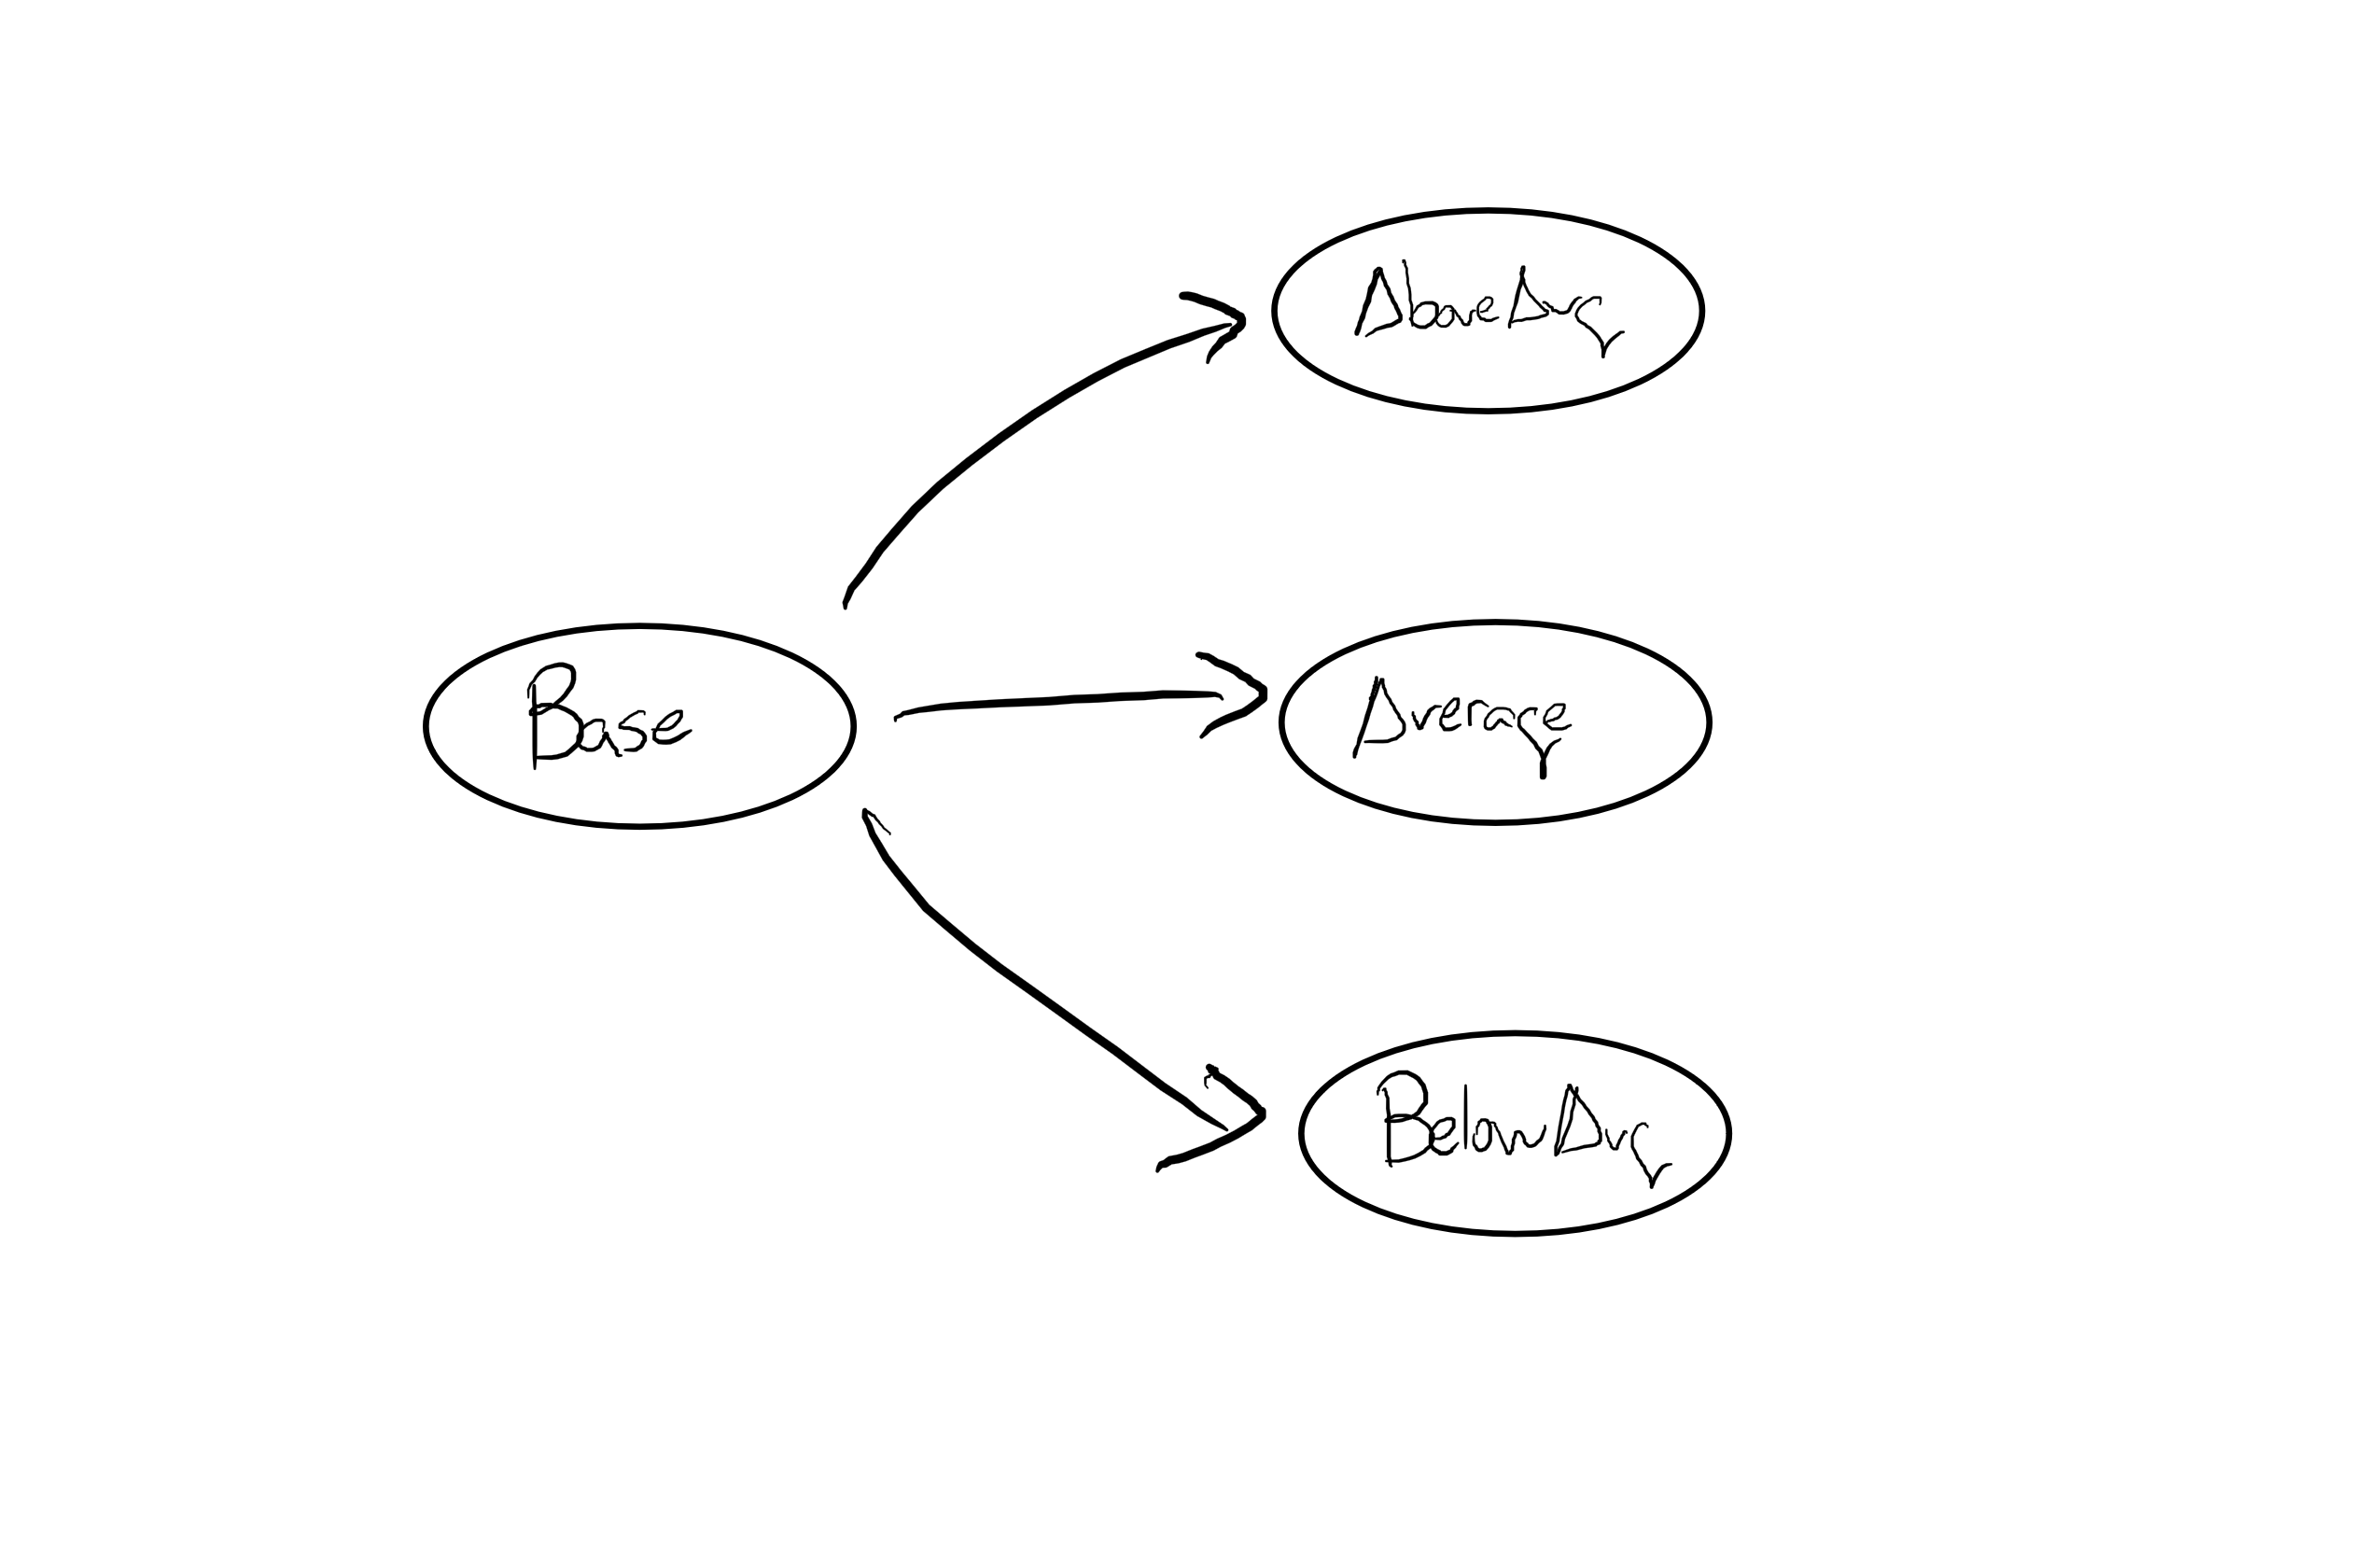
\includegraphics[width=15cm]{figuras/scenario-tree.png}}
    \caption{Árbol de escenarios en un problema estocástico}
    \label{fig:scenario-tree}
\end{figure}

Este tipo de problemas es muy común en el mundo real. Por ejemplo, en una tesis para la Universidad de Chile \cite{thesisHydro}, se utiliza la programación estocástica aplicada a la coordinación hidrotérmica. Este problema ``busca encontrar la operación óptima para un Sistema Eléctrico Mixto, combinando en la solución los efectos de las etapas futuras así como los efectos que la hidrología tiene en la operación del sistema''. Es un problema de optimización para una red energética gubernamental donde se deben tener en cuenta costes y eficiencia de cada tipo de generación de energía, además de contar con factores externos. \\

Los problemas estocásticos pueden subdividirse en problemas individuales (un problema para cada combinación de posibles escenarios generados) lo que los hace un claro objetivo de paralelización. Estos problemas individuales deben converger a una solución única, lo que se consigue con un algoritmo como el \textit{Progressive Hedging} el cual hace uso de las variables concretas de cada escenario y el valor de control $\rho$ para hacer converger las soluciones a un valor equivalente a la resolución del problema antes de subdividirlo.

\section{Motivación del proyecto}

% Adaptarse a nuevas tecnologías para abarcar problemas de mayor tamaño.

Como se ha explicado en el apartado anterior, los problemas estocásticos representan situaciones comunes y su solución puede ser aplicable a muchos campos diferentes. Además, Pyomo ya dispone de herramientas para solucionar este tipo de problemas de forma sencilla, siendo incluso posible hacerlo de forma paralela.\\

Este proyecto tiene como objetivo realizar una nueva implementación alternativa haciendo uso de herramientas Big Data como Spark o tecnologías como MPI. Esta implementación funcionará como base para la resolución de problemas estocásticos en entornos distribuidos, siendo susceptible de recibir optimizaciones concretas para la tecnología escogida y plataformas futuras.

\section{Estado del arte}

% Hablar de Big Data, su orientación principal al manejo de datos masivo. Haremos una adaptación a usarlo como motor de cálculo en entornos de computación distribuida.

Existen múltiples métodos para solucionar problemas estocásticos. Una forma es solucionar la ``representación extendida'' del problema. En este caso se preprocesa el árbol de escenarios para resolverlo como un problema único.\\

El método en el que se centrará este proyecto es el algoritmo ``Progressive Hedging'' que, como se explicó anteriormente, consiste en la solución de subproblemas y la convergencia de sus soluciones. Podemos ver el algoritmo concreto en \autoref{fig:ph_pseudocode}.\\

\begin{figure}
    \centerline{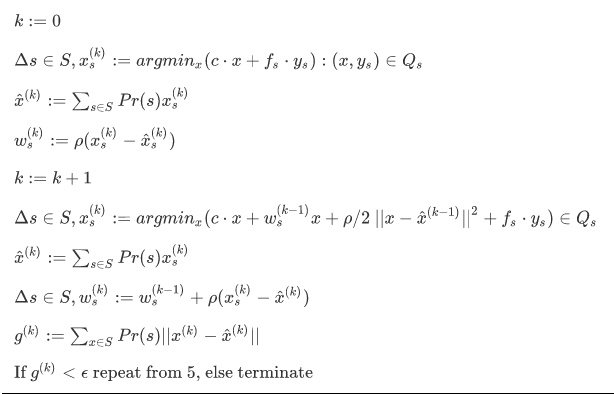
\includegraphics[width=15cm]{figuras/ph-pseudocode.png}}
    \caption{Pseudocódigo del algoritmo Progressive Hedging}
    \label{fig:ph_pseudocode}
\end{figure}

A continuación se especifican las posibles herramientas para implementar este algoritmo y Pyro, la librería utilizada en la implementación paralela ya existente en Pyomo.

\subsection{Big Data}

El término Big Data se refiere al manejo masivo de datos cada vez más relevante en los últimos años. El software orientado a Big Data está optimizado para la obtención, almacenamiento y procesamiento de grandes cantidades de datos que sería inviable analizar con software tradicional. \\

Estudiaremos la herramienta Spark de Apache para la implementación del algoritmo. Spark es un framework de código abierto para la programación en entornos distribuidos. Proporciona una capa de abstracción que permite ejecutar trabajos de forma distribuida sin tener conocimiento de las características del cluster. Spark se encarga de la distribución de los datos, el mantenimiento de su consistencia y la optimización de la repartición.\\

\subsection{MPI}

 MPI, siglas para \textit{``Message Passing Interface''}, es un estándar de paso de mensajes que permite la comunicación entre programas a través de la red. Esta interfaz puede utilizarse para implementar una red de objetos distribuidos y solucionar problemas de forma paralela.\\

 MPI permite el paso de mensajes utilizando tipos primitivos o la creación de tipos personalizados. La comunicación puede ser punto a punto entre dos objetos, sincronizando las llamadas a \textit{send} y \textit{receive}, o puede ser colectiva. MPI también provee funciones para facilitar la ejecución de algoritmos distribuidos como MPI\_BCAST, MPI\_SCATTER o MPI\_REDUCE.
 
\subsection{Pyro}

La intención de este proyecto es realizar una implementación paralela del algoritmo progressive hedging. Para cumplir este objetivo satisfactoriamente, debemos fijarnos en la implementación existente que, en este caso, utiliza la librería Pyro \cite{pyro}. \\

Pyro es una librería de Python para la implementación de objetos remotos. Funciona de una forma similar a RMI de Java, utilizando un servidor de nombres donde los objetos son registrados. Una vez hecho el lookup de un objeto remoto se puede utilizar como un objeto nativo de python, pero la ejecución se realizará sobre el objeto remoto.\\

Este tipo de comunicación entre objetos permite adaptar de forma sencilla un algoritmo implementado con una arquitectura basada en objetos a un entorno paralelo. Sin embargo, este tipo de comunicación tiene ciertas desventajas:

\begin{itemize}
    \item Se debe gestionar manualmente la repartición de trabajo en un entorno distribuido.
    \item No es sencillo optimizar la distribución de memoria entre los nodos de trabajo.
\end{itemize}

\section{Objetivos}

% Los objetivos expuestos en el anteproyecto: generar un módulo para Pyomo y evaluar su rendimiento.

El objetivo principal de este trabajo es paralelizar el algoritmo Progressive Hedging del módulo PySP. Este objetivo principal puede subdividirse en los siguientes objetivos específicos:

\begin{itemize}
    \item Estudiar y analizar el funcionamiento del algoritmo Progressive Hedging en PySP.
    \item Análisis de las diferentes alternativas de paralelización disponibles que mejor se adapten al problema. Se tendrán en cuenta tecnologías Big Data (Apache Spark) o modelos tradicionales (MPI).
    \item Diseño e implementación del nuevo módulo e integración con Pyomo.
    \item Análisis y evaluación del rendimiento.
\end{itemize}

\section{Estructura de la Memoria}

% Lista con los capítulos y qué se trata en cada uno de ellos.

En los siguientes apartados de este documento se especificará el desarrollo del proyecto necesario para el cumplimiento de los objetivos anteriores.

\begin{itemize}
    \item \textbf{\autoref{ch:gestion}: } Especifica aspectos relativos a la gestión del proyecto indicando alcance, requisitos, riesgos, costes y el cronograma del proyecto.
    \item \textbf{\autoref{ch:analisis}: } Describe el procedimiento de análisis del proyecto y las tecnologías necesarias.
    \item \textbf{\autoref{ch:implementacion}: } Explica el código desarrollado y los métodos utilizados para su implementación.
    \item \textbf{\autoref{ch:pruebas}: } Determina las pruebas a realizar sobre la implementación para establecer un nivel de confianza concreto sobre el funcionamiento del mismo. Adicionalmente, se establecerán medidas de rendimiento de la nueva implementación.
    \item \textbf{\autoref{ch:conclusiones}: } Resume las conclusiones extraidas de la realización del proyecto, lecciones aprendidas y trabajo futuro que ayudaría a mejorar el resultado final.
\end{itemize}
\cleardoublepage
\chapter{Gestión del proyecto}
\label{ch:gestion}

\section{Alcance}

\subsection{Descripción del alcance del proyecto}

En este proyecto se construirá un módulo software como parte del proyecto Pyomo. Este nuevo módulo adaptará el funcionamiento del actual módulo de programación estocástica (\textit{PySP}) a una implementación paralela.\\

Se realizará un estudio inicial de Pyomo para decidir la integración y la tecnología a utilizar para la nueva implementación. El objetivo de esta nueva implementación es el de proporcionar una ejecución más escalable que permita abordar problemas de mayor tamaño o, al menos, proporcionar una implementación base que, con futuras optimizaciones, permita conseguir ese objetivo.\\

El rendimiento de esta nueva implementación estará reflejado en un informe tras hacer pruebas con distintos problemas y en distintos sistemas.

\subsection{Criterios de aceptación}

El proyecto será aceptado cuando se superen las pruebas definidas en el \autoref{ch:pruebas}.\\

El proyecto persigue dos objetivos: la implementación del algoritmo en paralelo y un estudio de rendimiento. La nueva implementación debe ser capaz de resolver problemas estocásticos de forma paralela usando el algoritmo \textit{Progressive Hedging} y su rendimiento debe escalar añadiendo nodos de computación. Esta implementación debe poder ejecutarse sobre una instalación remota de Spark y utilizando como entrada los mismos modelos de problema que la versión actual de Pyomo. 

\subsection{Entregables del proyecto}

Los elementos a entregar tras la finalización del proyecto son:

\begin{itemize}
    \item Código de Pyomo actualizado con el módulo de ejecución de PH paralelo.
    \item Estudio de rendimiento (incluído en el documento actual).
    \item Memoria de realización del proyecto.
    \item Otra documentación asociada a la realización del proyecto.
\end{itemize}

\subsection{Exclusiones}

El proyecto producirá una implementación paralela del algoritmo PH existente. Esta implementación debe ser funcional pero no es un objetivo del proyecto hacer que esta nueva implementación sea mejor que la anterior en términos de eficiencia o rapidez.\\

Pyomo permite el uso de plugins externos que se pueden ejecutar antes o después de calcular la solución y pueden modificar la entrada/salida del mismo. No se harán pruebas de compatibilidad de la nueva solución con estos plugins de terceros en Pyomo. Sólo se verificará su funcionamiento con la ejecución incluida por defecto.

\subsection{Restricciones}

El proyecto debe finalizar el día 18/06/2018. En caso de ser necesario se puede postponer la fecha de finalización hasta el 27/07/2018.

\section{Análisis de requisitos}

El objetivo principal de este trabajo es el de paralelizar el algoritmo \textit{Progressive Hedging} del módulo PySP. Para conseguirlo se establecen los siguientes requisitos:

% TODO: Introducción a las tablas y concretar algo más. Introducción similar a lo explicado en la sección de riesgos.
% TODO: Añadir requisitos no funcionales y casos de uso.

\Req [
    id=RF-01,
    name={Ejecución de trabajos en Spark},
    description={Ejecutar el algoritmo PH en Spark de forma paralela.},
    priority={Imprescindible}
] { \caption{RF-01: Ejecución de trabajos en Spark}
    \label{tab:rf01}}

\Req [
    id=RF-02,
    name={Integración con Pyomo},
    description={La solución implementada debe funcionar como parte del programa Pyomo.},
    priority={Imprescindible}
] { \caption{RF-02: Integración con Pyomo}
    \label{tab:rf-02}}

\Req [
    id=RF-03,
    name={Interoperabilidad con funcionalidad previa},
    description={La nueva implementación no debe impedir el correcto funcionamiento de los módulos de Pyomo existentes.},
    priority={Importante}
] { \caption{RF-03: Interoperabilidad con funcionalidad previa}
    \label{tab:rf-03}}

\Req [
    id=RF-04,
    name={Establecer medición de rendimiento de Spark},
    description={Cuantificar la diferencia de rendimiento y escalabilidad de la nueva implementación.},
    priority={Importante}
] { \caption{RF-04: Establecer medición de rendimiento de Spark}
    \label{tab:rf-04}}

\section{Análisis de riesgos}

Para un proyecto del tamaño y duración estimados para este TFG es de vital importancia analizar los posibles riesgos que pueden poner en peligro la satisfactoria finalización del trabajo.\\

A continuación se especifican los potenciales riesgos junto a su probabilidad, impacto y tratamiento.\\

La probabilidad se medirá como:

\begin{itemize}
    \item \textbf{Muy alta:} Probabilidad de ocurrencia superior al 90\%.
    \item \textbf{Alta:} Probabilidad de ocurrencia superior al 70\%.
    \item \textbf{Moderada:} Probabilidad de ocurrencia superior al 40\%.
    \item \textbf{Baja:} Probabilidad de ocurrencia inferior al 40\%.
\end{itemize}

El impacto que tendrá la ocurrencia del riesgo sobre los activos afectados se medirá como:

\begin{itemize}
    \item \textbf{Catastrófico: } Supone la cancelación de tareas, inhabilidad de cumplir la fecha límite o, por último, la cancelación del trabajo.
    \item \textbf{Serio: } Supone modificaciones importantes pero asumibles en la realización de las tareas o el tiempo asignado a las mismas.
    \item \textbf{Tolerable: } La aparición del riesgo causará la necesidad de trabajo extra pero asumible. También puede suponer eliminar tareas o resultados poco importantes.
    \item \textbf{Irrelevante: } Las consecuencias generadas por el riesgo pueden ignorarse sin efectos demasiado negativos.
\end{itemize}

\RiskItem [
    id={R-01},
    name={Mala gestión del tiempo de realización del anteproyecto},
    description={
        Un anteproyecto erróneo puede suponer el rechazo del mismo. En menor medida, una descripción demasiado concreta puede suponer un limitante a la hora de realización del trabajo.
    },
    probability={Moderada},
    impact={Catastrófico},
    affected={Anteproyecto},
    treatment={Prevención -- Generar una lista de elementos necesarios para el anteproyecto, planificarlos temporalmente y cumplir dicha planificación.},
    indicators={No cumplir la planificación.},
    follow={Semanal.}
] { \caption{R-01: Mala gestión del tiempo de realización del anteproyecto}
    \label{tab:r-01}}

\RiskItem [
    id={R-02},
    name={No identificar correctamente los objetivos del trabajo},
    description={
        Unos objetivos poco claros pueden llevar a realizar trabajo innecesario o no realizar trabajo imprescindible. También pueden ocasionar desarrollo más lento por no saber qué hacer a continuación.
    },
    probability={Moderada},
    impact={Serio},
    affected={Anteproyecto, Planificación temporal, Código},
    treatment={Minimización -- Revisión de los objetivos dispuestos en el anteproyecto con el tutor del TFG. Esta revisión se hará con antelación suficiente para realizar cambios si fuesen necesarios.},
    indicators={Redacción poco clara del propósito del trabajo en la realización del anteproyecto.},
    follow={Semanal.}
] { \caption{R-02: No identificar correctamente los objetivos del trabajo}
    \label{tab:r-02}}

\RiskItem [
    id={R-03},
    name={Inhabilidad para ajustar el trabajo a las horas requeridas},
    description={
        La realización de un TFG tiene establecida una cantidad de horas fija. Su incumplimiento debe estar justificado.
    },
    probability={Alta},
    impact={Tolerable},
    affected={Planificación temporal},
    treatment={Minimización -- Se estimará la duración de las tareas al alza. En caso de que la planificación acabé con más horas de las permitidas, se podrá disminuir la duración de las tareas menos importantes.},
    indicators={La planificación suma más horas de las permitidas.},
    follow={Cada vez que se modifique la planificación.}
] { \caption{R-03: Inhabilidad para ajustar el trabajo a las horas requeridas}
    \label{tab:r-03}}

\RiskItem [
    id={R-04},
    name={Memoria final poco concreta},
    description={
        La memoria del proyecto debe representar fielmente el desarrollo del mismo. Si se retrasa demasiado su realización es posible perder detalles relevantes del proyecto.
    },
    probability={Alta},
    impact={Serio},
    affected={Memoria},
    treatment={Minimización -- Se realizarán, semanalmente o cada 15 días, documentos de progreso que especifiquen las tareas realizadas. Con esto se tendrá una documentación informal pero muy actualizada y concreta.},
    indicators={Parte del desarrollo no está especificado en ningún documento de progreso ni en la memoria final.},
    follow={Semanalmente.}
] { \caption{R-04: Memoria final poco concreta}
    \label{tab:r-04}}

\RiskItem [
    id={R-05},
    name={Incumplimiento del cronograma del proyecto},
    description={
        Por errores de código, inexperiencia o una carga de trabajo externa mayor de lo esperada, algunas tareas pueden durar más de lo planificado.
    },
    probability={Muy alta},
    impact={Serio},
    affected={Planificación temporal},
    treatment={Prevención -- Seguir el porcentaje de cumplimiento de las tareas sobre el cronograma.},
    indicators={Una tarea no se finaliza en plazo o el porcentaje de realización no es suficiente para el tiempo establecido en la tarea.},
    follow={Diario.}
] { \caption{R-05: Incumplimiento del cronograma del proyecto}
    \label{tab:r-05}}

\RiskItem [
    id={R-06},
    name={Incompatibilidad de la herramienta escogida con Pyomo},
    description={
        Se hará un estudio de herramientas para paralelizar el algoritmo. Si esta herramienta sufre algún tipo de incompatibilidad con el proyecto existente supondrá un retraso importante.
    },
    probability={Baja},
    impact={Catastrófico},
    affected={Diseño, Código},
    treatment={Prevención -- Durante la elección de la herramienta se harán pruebas sencillas sobre el proyecto. Tras crear el diseño se hará una implementación de prueba.},
    indicators={Aparecen errores en el programa que no son causados por fallos de programación.},
    follow={Semanal durante la fase de diseño. Cada 15 días durante la implementación.}
] { \caption{R-06: Incompatibilidad de la herramienta escogida con Pyomo}
    \label{tab:r-06}}

\RiskItem [
    id={R-07},
    name={Retraso del proyecto},
    description={
        Alguna de las tareas planificadas dura más de lo especificado. El impacto dependerá de la gravedad del retraso.
    },
    probability={Moderada},
    impact={Variable},
    affected={Todos los ECS},
    treatment={Minimización -- La planificación se creará con un margen de retraso proporcional a la complicación de la tarea.},
    indicators={Una tarea está tardando en finalizar más de lo esperado.},
    follow={Semanalmente.}
] { \caption{R-07: Retraso del proyecto}
    \label{tab:r-07}}

\RiskItem [
    id={R-08},
    name={No conseguir acceso a un cluster},
    description={
        Para probar el software es ideal utilizar un cluster de computación que permita evaluar la escalabilidad de la solución.
    },
    probability={Moderada},
    impact={Serio},
    affected={Memoria, Informe de rendimiento},
    treatment={Aceptar -- La pruebas se realizarán en un ordenador personal y es posible que tengan resultados menos relevantes.},
    follow={Al finalizar la implementación y al comenzar la ejecución de las pruebas.}
] { \caption{R-08: No conseguir acceso a un cluster}
    \label{tab:r-08}}

\section{Análisis de costes}

En esta sección se realizará un cálculo de los costes del proyecto basados en la planificación temporal establecida.\\

\subsection{Costes materiales}

En primer lugar se hará un cálculo de los costes materiales necesarios para la realización del proyecto.

El único material utilizado ha sido el ordenador de desarrollo. Considerando una vida útil de 4 años y un precio base de 800{\euro} el precio de su uso a lo largo de 78 días es:

\begin{equation}
    \frac{800}{365*4} * 78 = 42\mbox{\euro}
\end{equation}

Todo el software utilizado para la realización del proyecto es gratuito a excepción de MSProject, del cual se hizo uso de la licencia de prueba gratuita.

\subsection{Costes personales}

El coste del desarrollador se estima en 16.300{\euro} brutos. Deduciendo IRPF y costes de Seguridad social, se estima el coste por hora en 17{\euro}.\\

Se deben tener en cuenta los gastos que suponen las reuniones con el tutor del TFG. Se calcula un coste por hora de 28{\euro} y un tiempo total de reuniones en 25h.\\

Si el proyecto dura 78 días y está planificado para un trabajo diario de 5h, los costes personales son:\\

\begin{tabularx}{\linewidth}{|p{3cm}|X|}
    \hline
    \textbf{Desarrollador} & $17*78*5=6630\mbox{\euro}$ \tabularnewline
    \hline
    \textbf{Tutor} & $28*25=700\mbox{\euro}$ \tabularnewline
    \hline
\end{tabularx}

\subsection{Costes indirectos}

Estos costes no están directamente relacionados con el desarrollo del proyecto pero proveen bienes necesarios para la realización del mismo. Entre ellos se encuentran servicios básicos como electricidad e internet.\\

Durante la realización del proyecto se hace uso de estos servicios proporcionados por la universidad mediante el Servicio Universitario de Residencias. \\

Considerando que el proyecto supone 5h diarias, esto es un 13\% del tiempo de uso de dichos servicios. Por lo tanto, en 5 meses (teniendo en cuenta la realización del anteproyecto): 29,25{\euro}

\subsection{Costes tras la ampliación del proyecto}

Una vez modificada la fecha de finalización del proyecto contamos con un mes adicional de gastos. Este nuevo mes debe contar con nuevos gastos indirectos por residir en la vivienda personal, lo que también implica un coste de 10{\euro} por cada reunión que suponga un desplazamiento a Santiago.\\

Esta nueva fecha de finalización supone 40 días extra de gasto. \\

En cuanto a costes materiales, se sumarán 40 días al uso del ordenador, sumando 22{\euro} extra.\\

Los gastos personales, asumiendo otras 15h extra para el tutor:\\

\begin{table} [H]
    \begin{tabularx}{\linewidth}{|p{3cm}|X|}
        \hline
        \textbf{Desarrollador} & $17*40*5=3400\mbox{\euro}$ \tabularnewline
        \hline
        \textbf{Tutor} & $28*15=420\mbox{\euro}$ \tabularnewline
        \hline
    \end{tabularx}
    \caption{Costes personales del proyecto}
    \label{tab:costes-personales}
\end{table}
\ \\
En los gastos indirectos, el precio ahora es superior, contando 57{\euro} de conexión a internet a mayores del resto de facturas, manteniendo el 13\% de uso, suma otros 90{\euro} en los meses de Junio y Julio.\\

Adicionalmente, se consideran 3 reuniones en este periodo adicional, con un coste de 13{\euro} cada una.

\subsection{Resumen de costes}

\begin{table} [h]
    \begin{tabularx}{\linewidth}{|p{3cm}|X|}
        \hline
        \textbf{Personales} & 10.850{\euro} \tabularnewline
        \hline
        \textbf{Materiales} & 64{\euro} \tabularnewline
        \hline
        \textbf{Indirectos} & 158,25{\euro} \tabularnewline
        \hline
    \end{tabularx}
    \caption{Resumen de costes del proyecto}
    \label{tab:costes-resumen}
\end{table}
    \ \\
De esta forma determinamos un \textbf{coste total del proyecto} de 11.072,25{\euro}

\section{Gestión de la configuración}

Para especificar la Gestión de la Configuración de este proyecto primero debemos identificar los Elementos de Configuración de Software (ECS), es decir, los elementos que se verán afectados por esta Gestión de la Configuración.\\

Elementos de Configuración:
\begin{itemize}
    \item Proyecto de software.
    \item Memoria del proyecto.
    \item Anteproyecto.
    \item Documentos de análisis y diseño.
    \item Informes de progreso.
    \item Plantillas de documentos.
\end{itemize}

Para gestionar las diferentes versiones de estos elementos de configuración se creará un repositorio git alojado en Github. Este repositorio contendrá toda la documentación. Para añadir el proyecto de software se realizará un \textit{fork} del proyecto Pyomo original y se añadirá como un submódulo a nuestro repositorio base. \\

Las modificaciones sobre el software serán individuales por lo que no será necesario considerar técnicas de consistencia en trabajo colaborativo. Para los cambios que se realicen se crea una rama específica sobre el \textit{fork} del proyecto.\\

Para relacionar de forma concreta tareas de la planificación con cambios en el repositorio se utiliza un tablero en la plataforma \textit{Trello}. Estas tareas se reflejan en los informes de progreso del repositorio. Además, funciona como herramienta organizativa.

\section{Planificación temporal}

\subsection{Metodología de desarrollo}

% TODO: Explicar elección de cascada.

\subsection{EDT}

\begin{figure}[H]
    \centerline{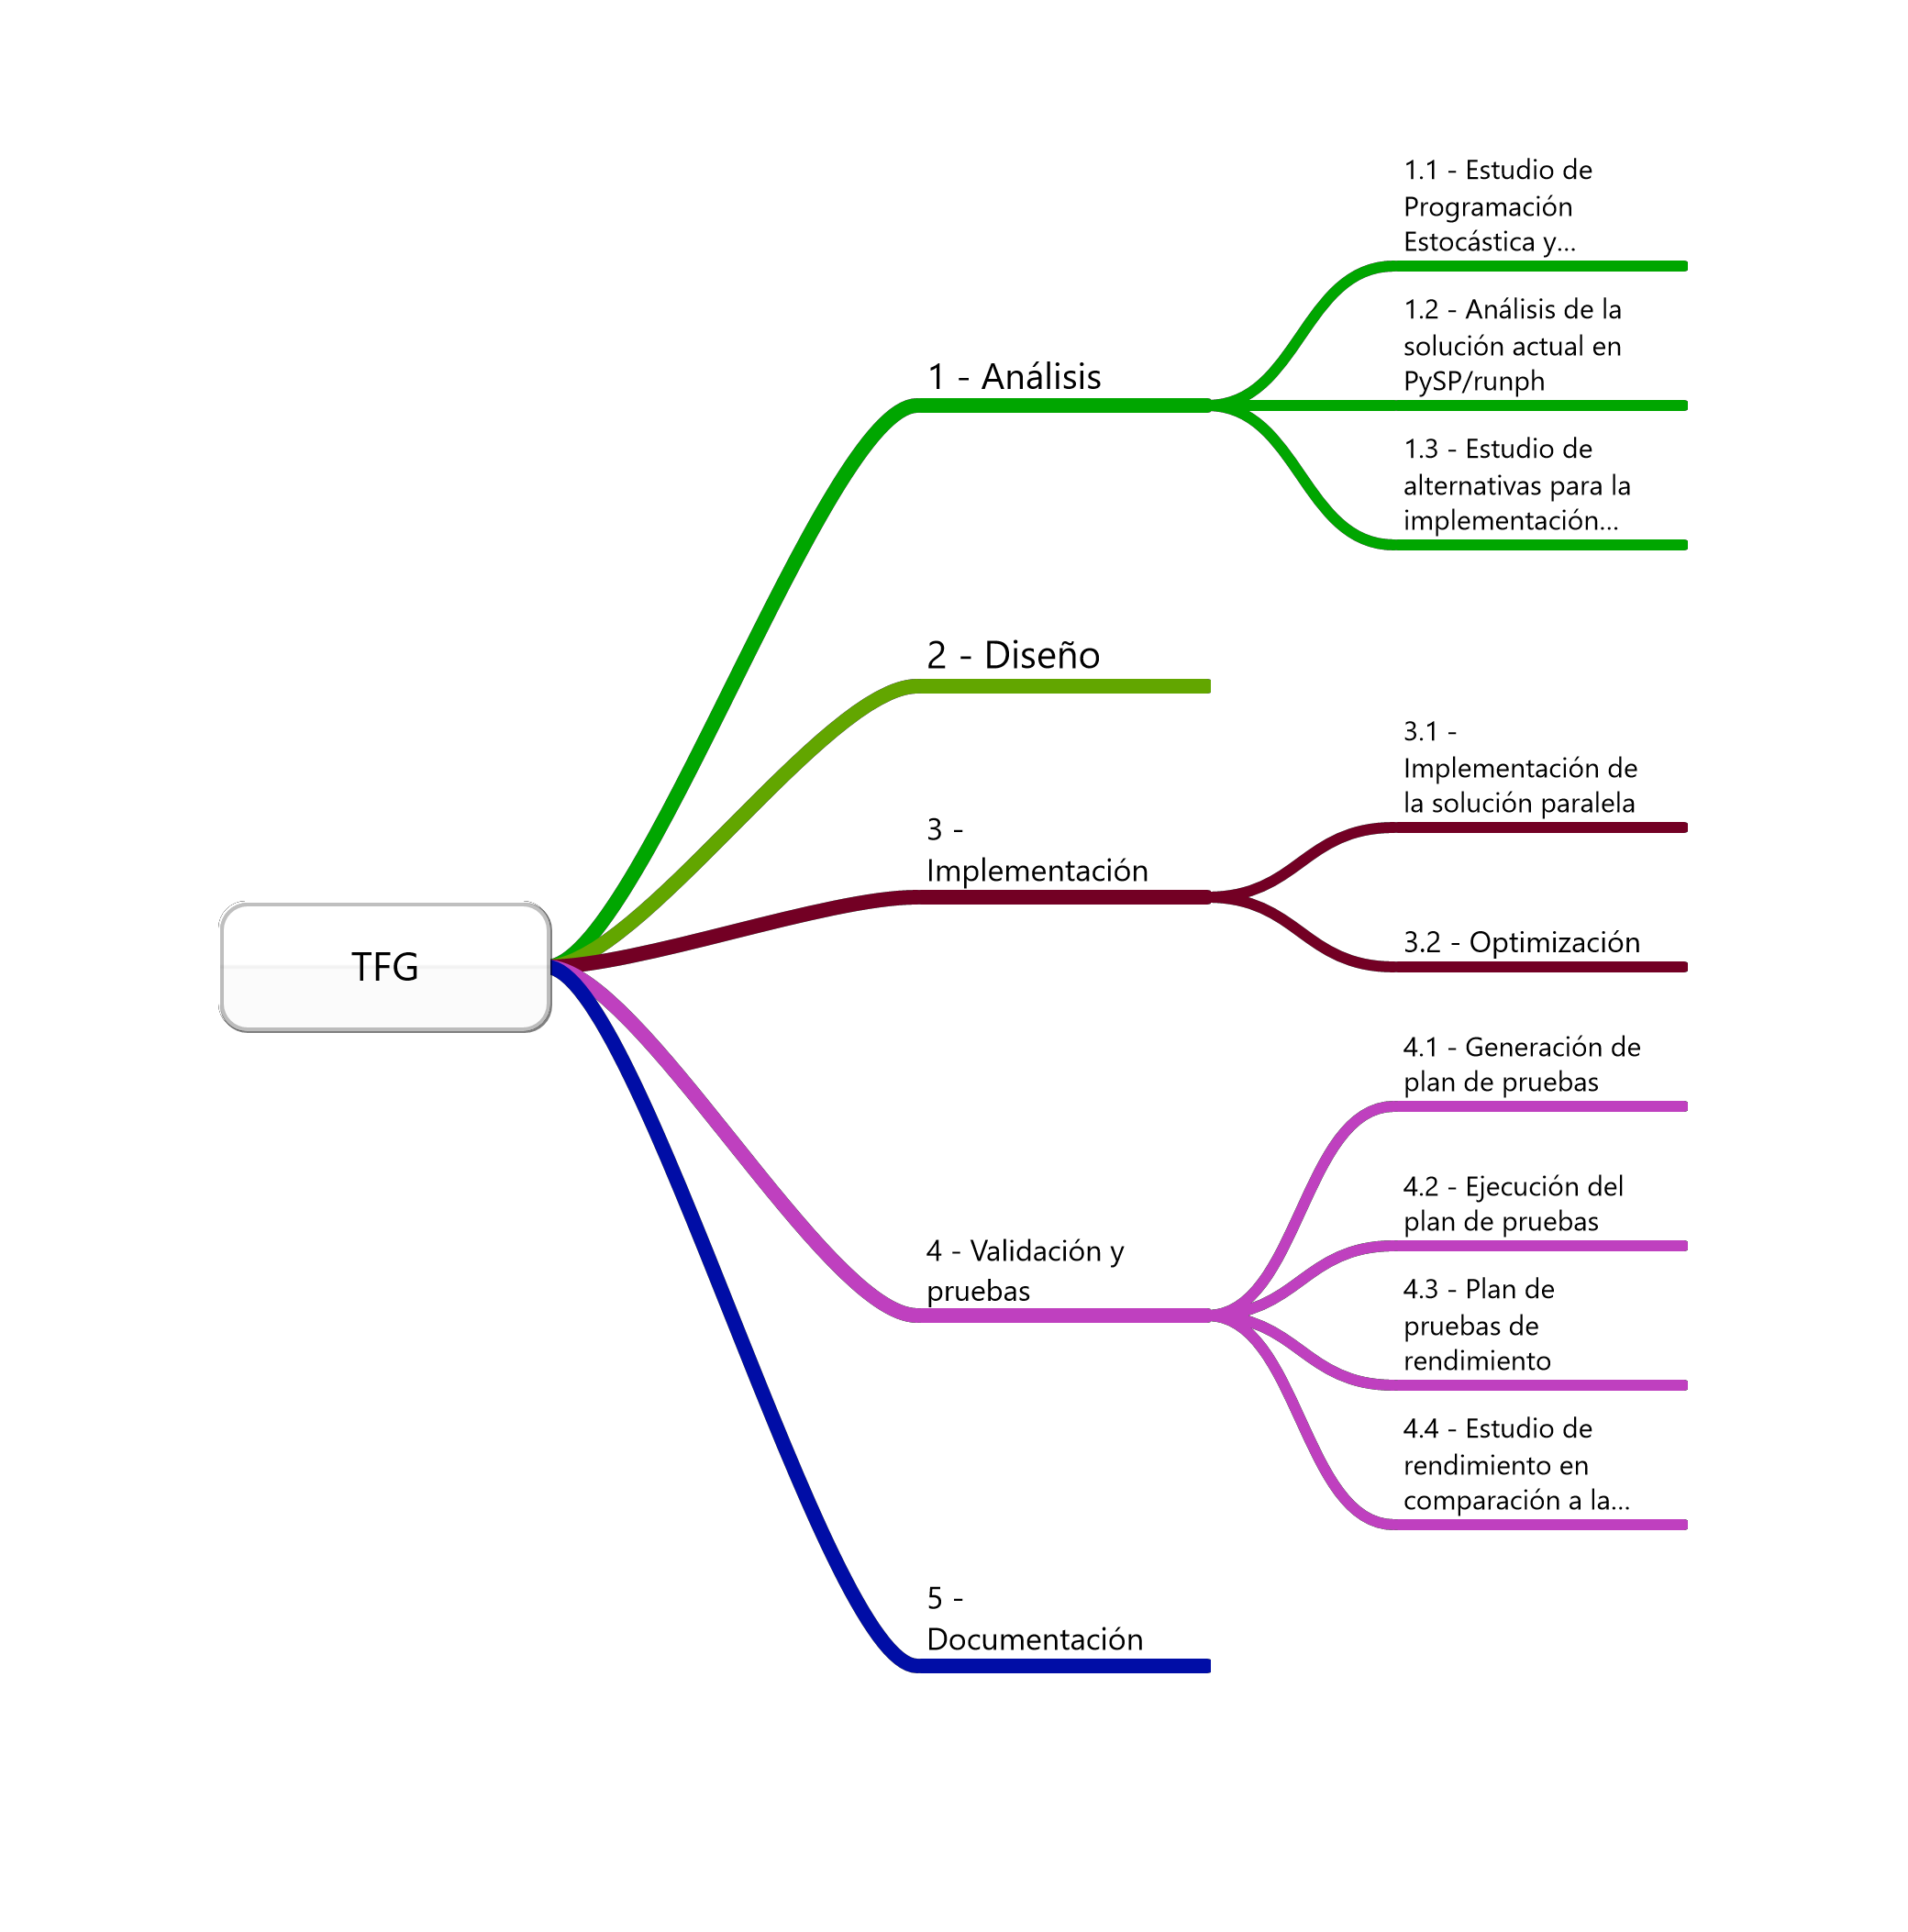
\includegraphics[width=15cm]{figuras/planificacion/edt-inicial.png}}
    \caption{EDT inicial}
\end{figure}

\WorkItem [
            id=1.1, 
            name={Estudio de Programación Estocástica y \textit{Progressive Hedging}},
            description= {
                Se investigará el funcionamiento del algoritmo {\it Progressive Hedging} haciendo uso principalmente de \cite{stochasticProgramming} como referencia.
            },
            duration=7,
            results={N/A}
        ]
{
    \caption{Tarea 1.1: Estudio de Programación Estocástica y \textit{Progressive Hedging}}
    \label{tab:task1.1}
}

\WorkItem [
        id=1.2, 
        name={Análisis de la solución actual en PySP/runph},
        description= {
            Una vez conocido el funcionamiento teórico del algoritmo, estudiar su implementación sobre el proyecto Pyomo.
        },
        duration=8,
        results={Diagrama de funcionamiento PH \cite{local_funcionamientoPH}.}
    ]
{
    \caption{Tarea 1.2: Análisis de la solución actual en PySP/runph}
    \label{tab:task1.2}
}

\WorkItem [
        id=1.3, 
        name={Estudio de alternativas para la implementación paralela},
        description= {
            Se barajarán tecnologías Big Data (Spark) o modelos tradicionales (MPI).
        },
        duration=3,
        results={Resultado del análisis en la \autoref{sec:herramientasAlternativas}}
    ]
{
    \caption{Tarea 1.3: Estudio de alternativas para la implementación paralela}
    \label{tab:task1.3}
}

\WorkItem [
        id=2, 
        name={Diseño},
        description= {
            Generar un diseño de la implementación a realizar con la tecnología escogida. Será importante la integración con la implementación actual.
        },
        duration=20,
        results={Diseño de la implementación.}
    ]
{
    \caption{Tarea 2: Diseño}
    \label{tab:task2}
}

\WorkItem [
        id=3.1, 
        name={Implementación de la solución paralela},
        description= {
            Escribir los nuevos módulos de código e integrarlos en el proyecto. 
        },
        duration=15,
        results={Nuevos ficheros de código y modificaciones a archivos existentes.}
    ]
{
    \caption{Tarea 3.1: Implementación de la solución paralela}
    \label{tab:task3.1}
}

\WorkItem [
        id=3.2, 
        name={Optimización},
        description= {
            Una vez la integración es correcta y la implementación funciona, se realizarán optimizaciones de rendimiento intentando aprovechar las carácterísticas de la tecnología escogida para la nueva implementación paralela.
        },
        duration=5,
        results={Modificaciones a la implementación anterior.}
    ]
{
    \caption{Tarea 3.2: Optimización}
    \label{tab:task3.2}   
}

\WorkItem [
        id=4.1, 
        name={Generación de plan de pruebas},
        description= {
            Idear un plan de pruebas para el nuevo módulo.
        },
        duration=4,
        results={Documento de pruebas \cite{local_planPruebas}.}
    ]
{
    \caption{Tarea 4.1: Generación de plan de pruebas}
    \label{tab:task4.1}
}

\WorkItem [
        id=4.2, 
        name={Ejecución del plan de pruebas},
        description= {
            Implementar y ejecutar las pruebas establecidas para establecer confianza sobre el correcto funcionamiento de la implementación.
        },
        duration=1,
        results={Informe de ejecución de pruebas.}
    ]
{
    \caption{Tarea 4.2: Ejecución del plan de pruebas}
    \label{tab:task4.2}
}

\WorkItem [
        id=4.3, 
        name={Plan de pruebas de rendimiento},
        description= {
            Idear un plan de pruebas con problemas que permitan estudiar el rendimiento del programa.  
        },
        duration=3,
        results={Documento de pruebas de rendimiento \cite{local_planPruebasRendimiento}.}
    ]
{
    \caption{Tarea 4.3: Plan de pruebas de rendimiento}
    \label{tab:task4.3}
}

\WorkItem [
        id=4.4, 
        name={Estudio de rendimiento},
        description= {
            Ejecutar el plan de pruebas anterior y compararlo con las versiones originales tanto secuencial como con Pyro.
        },
        duration=2,
        results={Informe de rendimiento \cite{local_informeRendimiento}.}
    ]
{
    \caption{Tarea 4.4: Estudio de rendimiento}
    \label{tab:task4.4}
}

\WorkItem [
        id=5, 
        name={Documentación},
        description= {
            Generar los documentos asociados al desarrollo del proyecto.
        },
        duration=10,
        results={Memoria del proyecto y documentos asociados.}
    ]
{
    \caption{Tarea 5: Documentación}
    \label{tab:task5}
}

\subsubsection{Tareas no planificadas}

Tras las modificaciones realizadas sobre el cronograma y explicadas en \autoref{sec:modificacionesCronograma}, se generan nuevas tareas para el proyecto: 
 
\WorkItem [ 
        id=3.*,  
        name={Prototipo aislado}, 
        duration=10, 
        description= {
            Crear una aplicación en Python que interactúe con Spark de forma similar a como lo hará la implementación en Pyomo. 
        }
    ] 
{ 
   \caption{Tarea 3.*: Prototipo aislado}
   \label{tab:task.3.*1}
} 
 
\WorkItem [ 
        id=3.*,  
        name={Prototipo de integración inicial}, 
        description= {
            Comenzar la implementación sobre Pyomo comprobando que la integración del nuevo módulo con el código existente es correcta y el flujo de ejecución es correcto con respecto al funcionamiento anterior. 
        },
        duration=5, 
        results={Código añadido a Pyomo.} 
    ] 
{ 
    \caption{Tarea 3.*: Prototipo de integración inicial}
    \label{tab:task3.*2}
} 
 
\WorkItem [ 
        id=3.*,  
        name={Prototipo funcional}, 
        description= {
            Modificar el prototipo anterior añadiendo las funcionalidades esperadas del programa.
        },
        duration=10, 
        results={Código añadido a Pyomo.} 
    ] 
{ 
     \caption{Tarea 3.*: Prototipo funcional}
     \label{tab:task3.*3}
} 

\subsection{Cronograma inicial}

Para la realización del trabajo se plantea un ciclo de vida en cascada. Este ciclo de vida nos permitirá realizar un seguimiento del progreso del proyecto en función del tiempo disponible.

\begin{figure}[H]
    \centerline{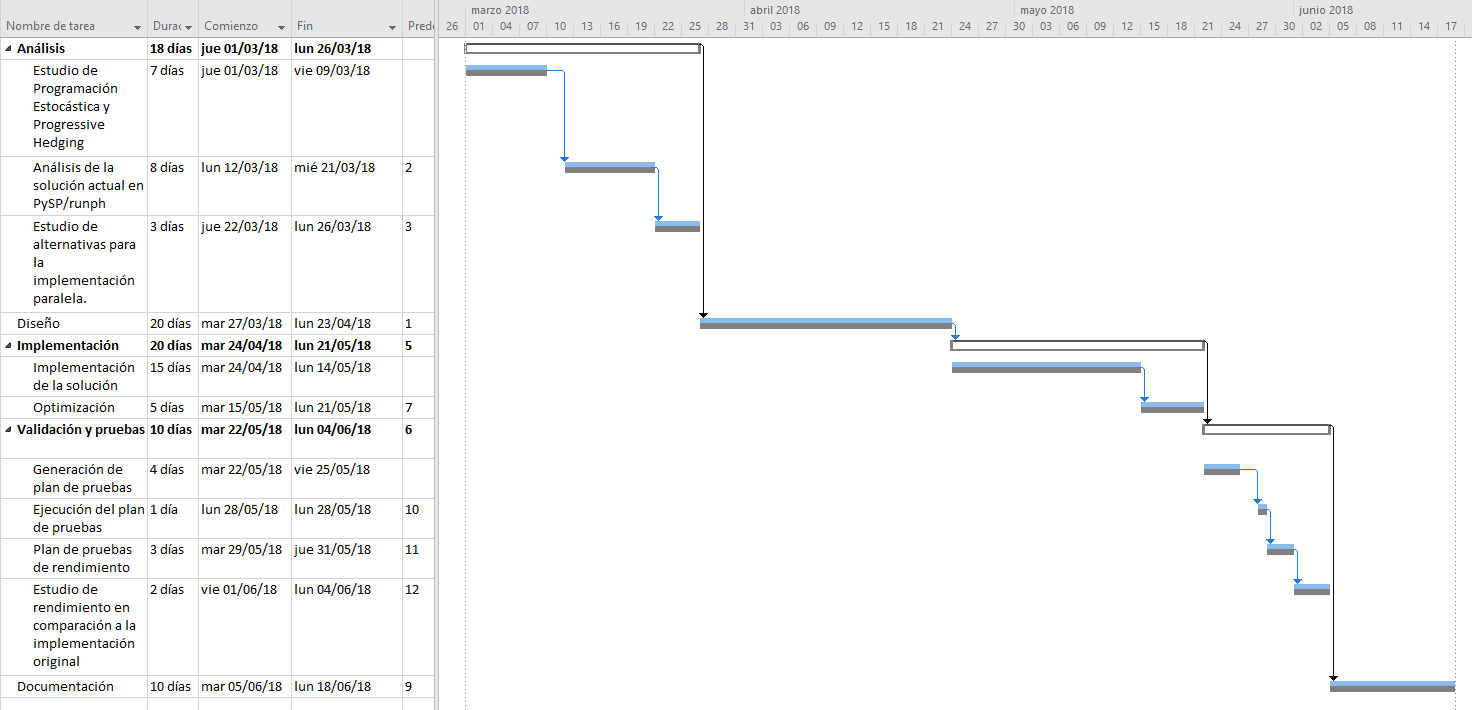
\includegraphics[width=18cm]{figuras/planificacion/linea-base.png}}
    \caption{Línea base}
\end{figure}

\subsection{Modificaciones al cronograma inicial}
\label{sec:modificacionesCronograma}

Se ha realizado una estimación temporal inicial poco precisa por no utilizar ningún tipo de método probado ni datos concretos.

Esta es la razón principal para los retrasos que se explican a continuación.

\subsubsection{Retraso en análisis}

El primer retraso se produce en la fase de análisis de la implementación actual. En esta fase se debe estudiar el funcionamiento del proyecto Pyomo y, en concreto, el módulo de resolución de problemas mediante \textit{Progressive Hedging}. 

A pesar de conocer el funcionamiento teórico del algoritmo mediante \cite{progressiveHedging}, Pyomo es un proyecto complejo, con multitud de funcionalidades para resolver otros tipos de problemas, soporte para plugins, etc. Todo esto hace que la complejidad del código aumente y sea necesario estudiar múltiples capas de abstracción para entender correctamente el funcionamiento del programa.

Otra complicación añadida es el personal desconocimiento del lenguaje Python previo a la realización de este trabajo.\\

Tras este primer retraso se intenta ajustar la planificación reduciendo el tiempo de diseño a la mitad:

\begin{figure}[H]
    \centerline{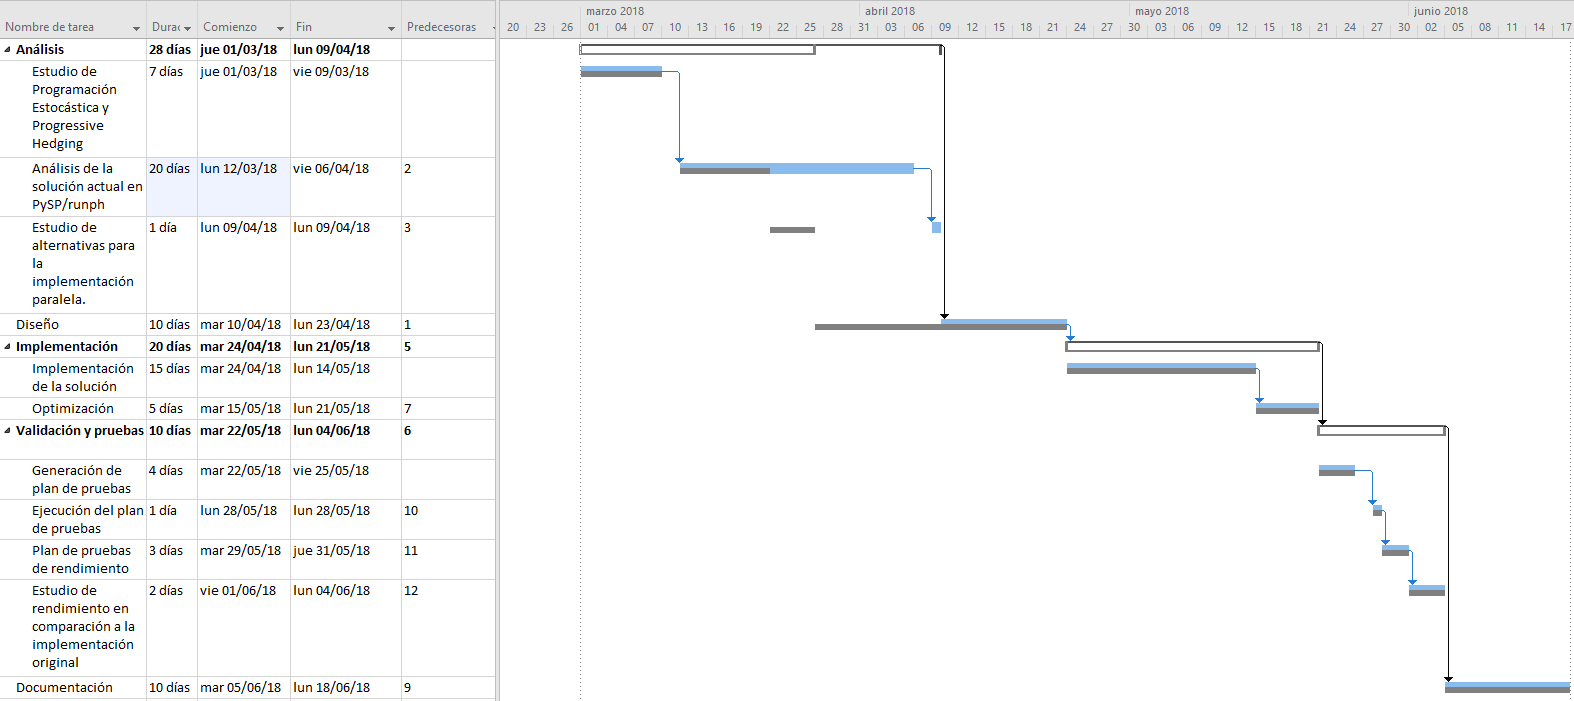
\includegraphics[width=18cm]{figuras/planificacion/1_retraso-analisis-inicial.png}}
    \caption{Primer retraso}
\end{figure}

Teniendo en cuenta que los primeros retrasos fueron principalmente causados por el desconocimiento de la tecnología a usar así como de una mala estimación, es muy probable que en las fases siguientes se produzcan otros retrasos. En este punto se considera entonces abandonar el ciclo de vida en cascada. Su principal atractivo era poder ajustarnos a una planificación temporal que nos permita acabar el proyecto dentro de tiempo, pero esta ventaja no se está cumpliendo en la práctica. Buscando reducir el tiempo de implementación con tecnologías que serán usadas por primera vez, se decide adaptar la planificación a un ciclo de vida por prototipos. 

La creación de sucesivos prototipos permite ir acostumbrándose a las tecnologías desconocidas, en este caso Python y Spark, así como ir probando el rendimiento y la integración a medida que se desarrolla.

En primer lugar se crea un prototipo aislado para comprobar la implementación de Spark con una arquitectura similar a la que se implementará en Pyomo. Este primer prototipo sirve como aprendizaje de la instalación de Spark y el despliegue de una aplicación en el mismo, así como la implementación en Python que interactuará con Spark. Es deseable utilizar una arquitectura de objetos Python similar a la que se usará en Pyomo para concretar el uso de Spark y descubrir posibles problemas con la implementación elegida.

Posteriormente se realizarán prototipos sucesivos sobre Pyomo para integrar el nuevo módulo e ir solucionando posibles problemas de rendimiento o funcionamiento que vayan surgiendo. 

Dado que la implementación partirá de un protipo inicial de baja calidad será importante realizar una fase de optimización y refactorización al final de la implementación para asegurarse un código final de calidad. Definir la calidad del código no es algo trivial y en este caso calificaremos el código como "de calidad" si cumple:

\begin{itemize}
    \item Funciona correctamente y es resistente a errores. Para esto nos apoyaremos en un plan de pruebas funcional.
    \item Funciona eficientemente y otorga un buen rendimiento, en comparación a las implementaciones existentes. En este caso nos apoyaremos en el plan de pruebas de rendimiento.
    \item Se integra adecuadamente al proyecto actual. Debe seguir una filosofía de diseño análoga al resto del código así como funcionar correctamente de forma paralela a todo lo implementado previamente.
\end{itemize}

Tras esta modificación en la planificación, se genera una nueva planificación que podemos ver en la figura y se guardará como una nueva línea base.

\begin{figure}[H]
    \centerline{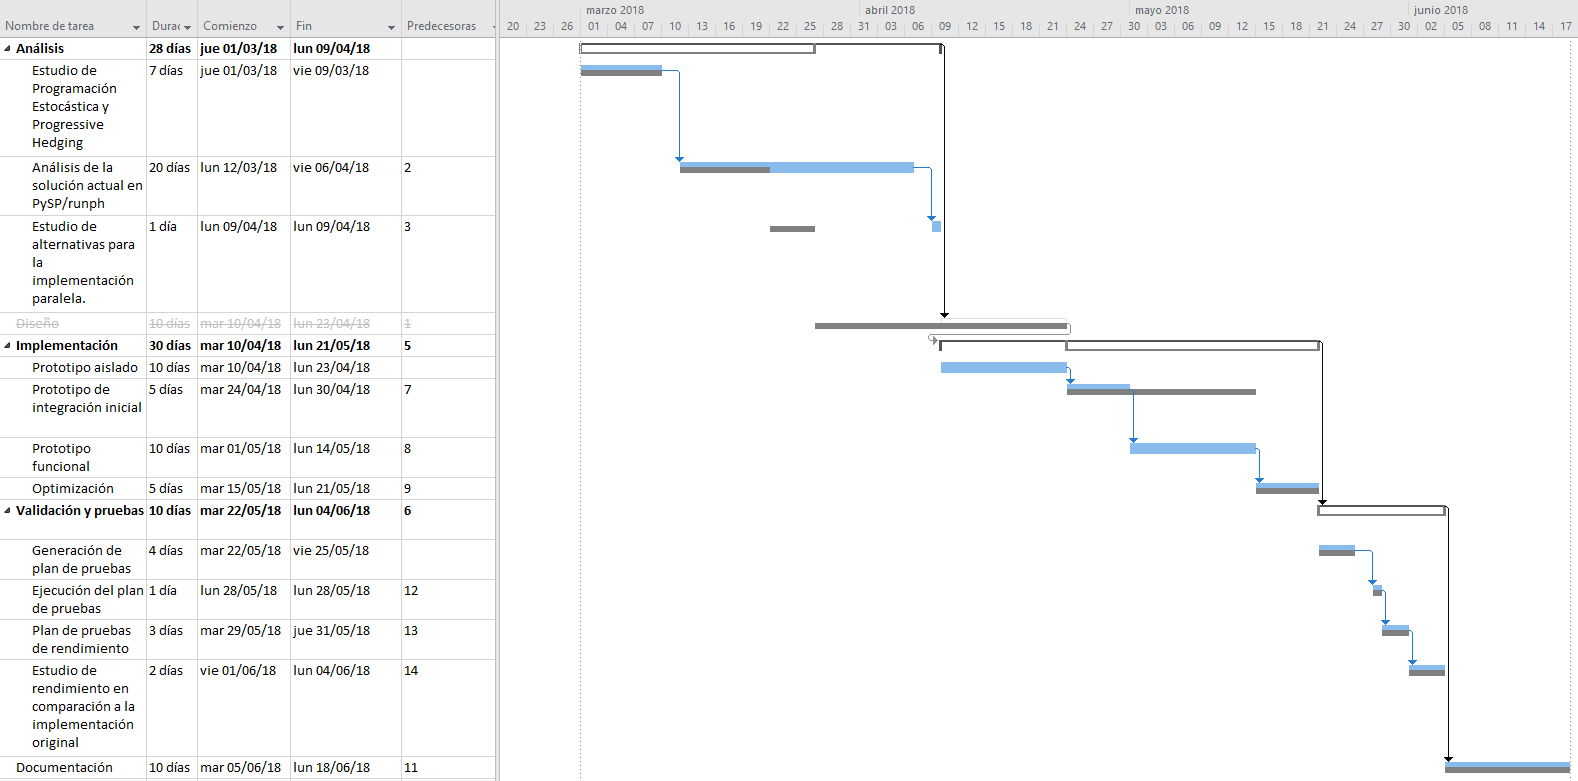
\includegraphics[width=18cm]{figuras/planificacion/2_linea-base-prototipos.png}}
    \caption{Línea base prototipos}
\end{figure}

En este punto hemos eliminado la fase de Diseño para poder aumentar el tiempo asignado a Análisis e Implementación. En caso de sufrir más retrasos en la fase de implementación podremos reducir el tiempo asignado a pruebas si el retraso no es grave. En caso de ser un retraso mayor, no cumpliremos la fecha de finalización establecida.

\subsubsection{Retraso en implementación}

Durante la implementación del prototipo funcional el desarrollo llega a un punto muerto. Las funciones implementadas no devuelven el resultado correcto y se debe hacer una búsqueda de los errores que lo causan. Por falta de experiencia y desconocimiento de las tecnologías, esta fase de implementación se alarga hasta el día 07/07/2018. \\

Este retraso sumado a un retraso de 10 días en la creación del prototipo aislado nos fuerza a retrasar la fecha de finalización del proyecto al día 25/07/2018. \\

Con estos nuevos cambios es necesaria una nueva planificación temporal:

\begin{figure}[H]
    \centerline{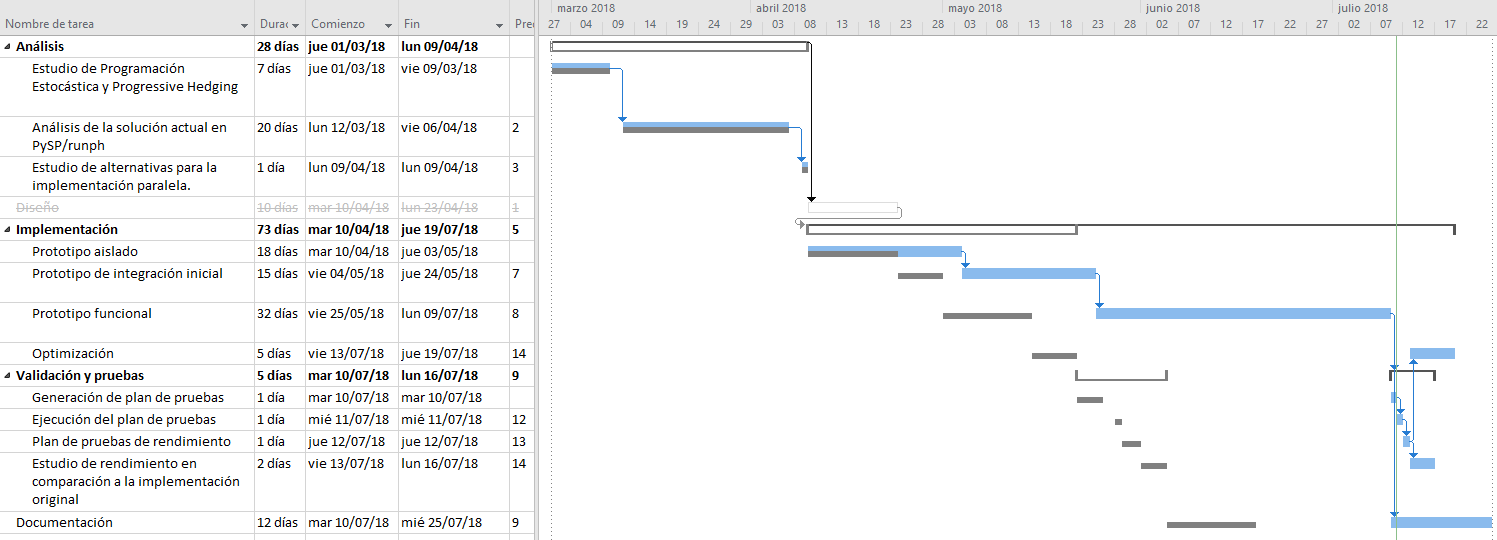
\includegraphics[width=18cm]{figuras/planificacion/3_linea-base-final.png}}
    \caption{Línea base final}
\end{figure}


\cleardoublepage
\chapter{Análisis}
\label{ch:analisis}

\section{Funcionamiento del algoritmo \textit{Progressive Hedging}}

% Explicación del algoritmo a nivel conceptual basándose en el libro de referencia de Birge.

El primer paso imprescindible para la realización de este proyecto será entender el algoritmo con el que se trabajará. Se debe estudiar el funcionamiento teórico de la Programación Estocástica y el algoritmo \textit{Progressive Hedging} con el objetivo de entender posteriormente su implementación en PySP. \\

Como referencia principal se utiliza el libro {\it Introduction to Stochastic Programming} \cite{stochasticProgramming}. Como se explicó anteriormente, la programación estocástica resuelve problemas donde existe un cierto nivel de incertidumbre. A lo largo de esta fase de análisis utilizaremos el ejemplo ``Farmer'' para ver un problema real en funcionamiento que sea sencillo de entender. Este problema está explicado en el libro anterior e incluido como ejemplo en el repositorio de Pyomo por lo que será una referencia muy útil.\\

En el problema del granjero, nos encontramos con una superficie concreta donde podemos plantar 3 tipos diferentes de cultivos. El problema de optimización es especificar la cantidad de superficie óptima para cada uno de los cultivos. Para llegar a la solución óptima se deben tener en cuenta múltiples restricciones como el precio por tonelada de cada cultivo, la cantidad de cultivo que conseguimos por unidad de superficie, su coste o cantidad mínima necesaria para venderlo. La incertidumbre en este problema viene dada por la eficiencia de cada cultivo. Aunque plantemos una cantidad concreta en una superficie específica, no podemos asegurar la cantidad de producto que conseguiremos pues depende de multitud de factores externos. Conocemos por datos pasados una aproximación de lo que producirá una cierta plantación, pero debemos considerar los escenarios en que esta producción será menor o superior. Con esto, tenemos un árbol de escenarios como el explicado en la \autoref{fig:scenario-tree}.\\

Para resolver este tipo de problemas, se utilizará el algoritmo \textit{Progressive Hedging}. Este algoritmo se ejecuta iterativamente y funciona descomponiendo el árbol de escenarios en problemas individuales. Cada rama del árbol se transforma en un problema lineal que se puede procesar directamente para obtener un resultado. Si simplemente hacemos esta descomposición y resolución, tendremos múltiples soluciones diferentes en función de los escenarios que existían en cada camino. Para poder obtener una solución correcta que tenga en cuenta todos los escenarios, debemos conseguir que todas las soluciones individuales convergan a un mismo valor (considerando un cierto margen de error). Esta convergencia se consigue iterando sobre el procesamiento de estos subproblemas. Evidentemente debemos hacer modificaciones en los mismos para poder conseguir la convergencia. Entre cada iteración se van a modificar las variables de las que depende cada subproblema siguiendo la fórmula definida por el algoritmo. El parámetro principal es la variable $\rho$, que no es específica de ningún problema. Esta variable se puede denominar como ``penalizador'' que influirá en cómo se modifican el resto de variables para hacer que sus valores tiendan a la solución buscada.
% TODO: explicar algoritmo

\begin{figure}
    \centerline{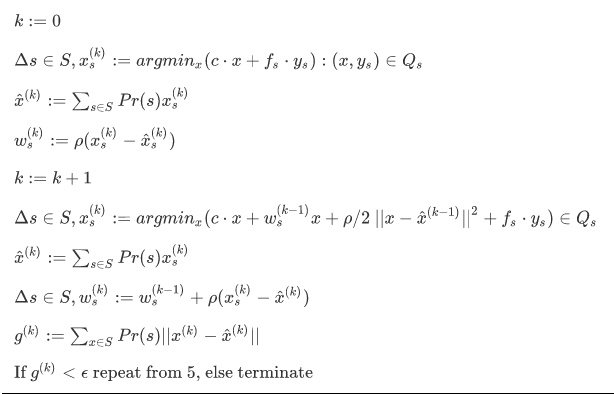
\includegraphics[width=15cm]{figuras/ph-pseudocode.png}}
    \caption{Pseudocódigo del algoritmo \textit{Progressive Hedging}}
    \label{fig:ph_pseudocode}
\end{figure}

\section{Analizando Pyomo}

% Cómo desplegar el proyecto para ver como funciona. Usaremos el ejemplo Farmer visto en el punto anterior.
% Procedimiento de análisis utilizando la salida --verbose y apoyándose en los apuntes de Onenote.

Una vez entendido el funcionamiento teórico del algoritmo, procedemos a ver la implementación del mismo en Pyomo. Podemos acudir a la propia documentación de PySP para hacernos una idea inicial de su funcionamiento. En este documento \cite{local_pyspdoc} se especifica cómo ejecutar el algoritmo mediante el comando \texttt{runph}. También especifica cómo utilizar Pyro para resolver el problema de forma paralela.\\

En este punto, necesitamos desplegar el proyecto para poder verlo en funcionamiento. El entorno sobre el que trabajaremos es el siguiente:

\begin{itemize}
    \item Para trabajar con el código se ha realizado un \textit{fork} del proyecto original en GitHub.
    \item Como IDE se utilizará PyCharm sobre Fedora 27.
    \item El código funcionará sobre un entorno virtual de Python 3.6 creado específicamente para este proyecto.
\end{itemize}

El primer paso será establecer una configuración de ejecución para el ejemplo \textit{Farmer}. Pyomo incluye una opción \texttt{--verbose} que proporciona una salida muy detallada de la ejecución y será extremadamente útil para este análisis, sobre todo, analizando la ejecución con Pyro.

Pyomo define comandos concretos para la ejecución de sus distintos módulos así que debemos buscar cuál es el punto de entrada del comando \texttt{runph}. Vemos que se utiliza un lenguaje de etiquetas personalizadas \texttt{@pyomo\_command} para definir estos puntos de entrada concretos. Si queremos ejecutar estos comandos desde el IDE, debemos hacer una modificación al archivo que queramos ejecutar para hacerlo ejecutable como script. En este caso, el archivo \textit{phinit.py} es el punto de entrada del método \texttt{runph}:

\begin{figure}[H]
    \centerline{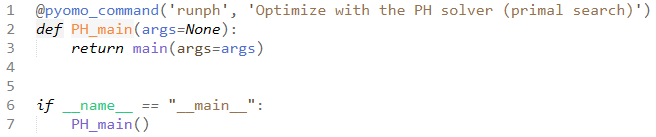
\includegraphics[width=15cm]{figuras/codigo/runph-command.png}}
\end{figure}

Con esta modificación podemos ejecutar el archivo como un script y será equivalente a ejecutar el comando \texttt{runph}. Podemos crear una configuración de ejecución en el IDE y usar la ejecución paso a paso para tener una visión general de la implementación. \\

Usando una herramienta incluida en PyCharm, podemos generar un árbol visual de llamadas a métodos. Esto genera la imagen \autoref{fig:call-tree} que representa el flujo que sigue la ejecución secuencial del algoritmo PH.

\begin{figure}[]
    \centerline{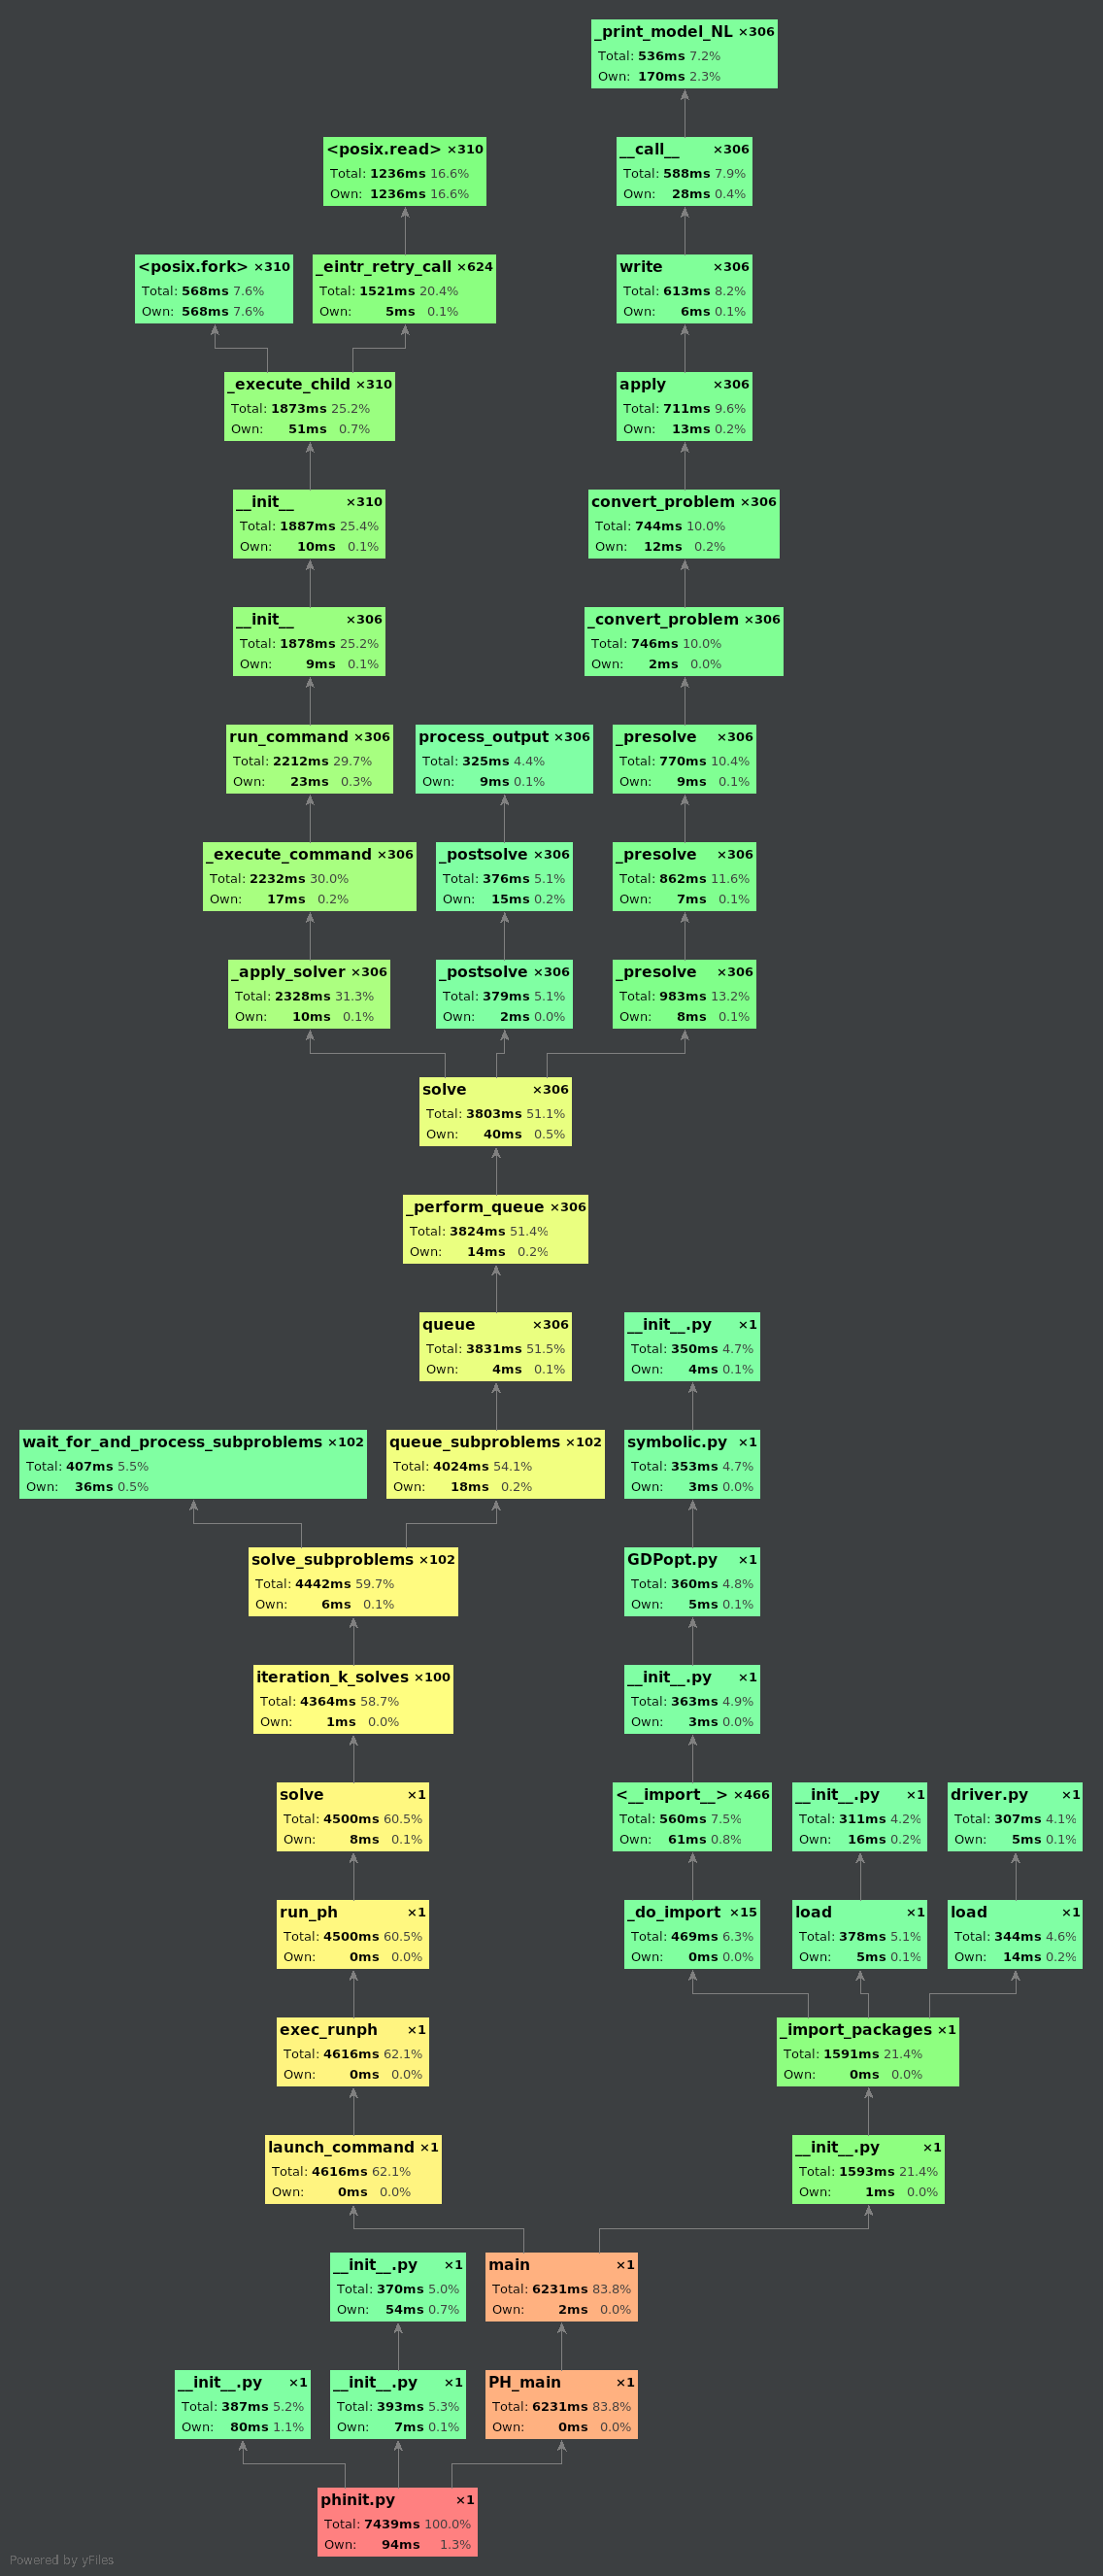
\includegraphics[width=10cm]{figuras/analisis/call-tree.png}}
    \caption{Árbol de llamadas en runph}
    \label{fig:call-tree}
\end{figure}

Podemos ignorar la rama de la derecha que se limita a la inicialización de los módulos Python. Lo relevante comienza en el método \texttt{run\_ph}. Vemos que se ejecuta el método \texttt{iteration\_k\_solves} y, aunque no está especificado en el diagrama, existe un método similar para la iteración 0, pues esta primera iteración es diferente al resto en el algoritmo PH.
En el siguiente paso observamos la primera decisión de diseño importante, se utiliza una cola para solucionar los problemas. Para cada subproblema especificado en el árbol se genera una tarea y se pone en cola. En un segundo método, se espera por los resultados. En esta ejecución secuencial esto no es muy relevante, pero lo será cuando veamos la implementación paralela.\\

En cuanto a la ejecución de la resolución, podemos distinguir tres fases: presolve, solve y postsolve:

\begin{itemize}
    \item En el \textbf{presolve} se preprocesan los escenarios del problema y se escriben en un archivo con el formato especificado. En este caso se escribe un archivo con el formato ``nl'' (\texttt{\_print\_model\_NL}) aceptado por solvers que siguen la interfaz AMPL \cite{AMPL}.
    \item En \textbf{\_apply\_solver} se utiliza el archivo generado en el paso anterior y la ruta al ejecutable del solver escogido (en nuestro caso usaremos ``minos'' \cite{minos}) para crear un comando. Esto se ejecuta como un comando en el sistema operativo y Python recoge el resultado.
    \item En el \textbf{postsolve} se procesa la salida recuperada del solver y se adapta en función del formato de salida.
\end{itemize}

En el método \texttt{solve} de \texttt{runph} es donde podemos encontrar el bucle principal que solicita al solver externo el resultado de cada iteración y realiza los cálculos necesarios para modificar los valores de cada subproblema. Al final de cada iteración se hace una prueba de convergencia que será la que indique la finalización del algoritmo.\\

Para nuestra implementación paralela analizaremos a continuación la implementación actual con Pyro. En este caso, por ser necesario lanzar múltiples procesos a la vez (el servidor de nombres, el propio \texttt{runph} y los workers), no podemos utilizar la ejecución paso a paso del IDE. En esta fase del análisis haremos usaremos la salida generada por la ejecución que, como dijimos antes, puede ser bastante específica haciendo uso de la opción \texttt{--verbose}. Analizando esta salida, podemos generar una traza con las operaciones realizadas:\\

\begin{itemize}
    \item Import model \& scenario.
    \item Construct solver manager.
    \item Construct solver.
    \item Wait for n servers to initialize.
    \item Instance each scenario.
    \item Post-instance-creation PHSolverServer plugins.
    \item Post-initialization PHSolverServer plugins.
    \item Post-initialization PH plugins.
    \item \textbf{Start PH}
    \begin{itemize}
        \item Iteration 0.
        \begin{itemize}
            \item Sync fixed variable status.
            \item Queue each solve for each scenario.
            \item Wait for scenario sub-problem solves.
            \item Pre-iteration-0-solve PHSolverServer plugins.
            \item Solve scenarios.
            \item Load all solutions.
            \item Post-iteration-0-solve PHSolverServer plugins.
            \item Convergence test.
            \item Transmitting request to activate PH objective proximal terms to PH solver servers.
            \item Transmitting request to activate PH objective weight terms to PH solver servers.
        \end{itemize}
        \item Iteration k.
        \begin{itemize}
            \item Sync fixed variable status.
            \item Transmit xbars.
            \item Transmit weights.
            \item Transmit rhos.
            \item Queue solve for each scenrio.
            \item Wait for scenario sub-problem solves.
            \item Pre-iteration-k-solve PHSolverServer plugins.
            \item Solve scenarios.
            \item Load all solutions.
            \item Post-iteration-k-solve PHSolverServer plugins.
        \end{itemize}
    \end{itemize}
\end{itemize}

En esta traza vemos la importancia que tiene el uso de una cola en la resolución de los problemas de forma paralela. El hilo principal pondrá tareas en esta cola y estas serán distribuidas a los distintos nodos de trabajo. Debemos identificar los objetos que están llevando esto a cabo. El objeto \texttt{PHSolverServer} es el encargado de ejecutar la resolución de cada subproblema y todas las tareas que se le pasen desde el hilo principal. Tendremos una instancia de este objeto por cada subproblema a resolver. En el ejemplo del \textit{Farmer}, como disponemos de 3 escenarios, tendremos tres instancias de \texttt{PHSolverServer} trabajando en paralelo. A estos objetos que realizan el trabajo en paralelo se los denominará normalmente como \textit{workers} a lo largo de este trabajo. El otro objeto relevante es el solver manager. Este objeto es el que define la distribución del trabajo. En el caso de la ejecución secuencial se utiliza \texttt{--solver-manager=serial} y, en este ejemplo, \texttt{--solver-manager=phpyro}. El solver manager se encarga de gestionar la cola de trabajos y especifica cómo se ejecutan.\\

En la traza anterior podemos observar claramente la comunicación entre el hilo principal y los workers. En cada iteración se solicita la resolución de un problema y se recoge su solución. Con esta solución se calculan las nuevas variables de control que serán retransmitidas al principio de la siguiente iteración. \\

Llegados a este punto tenemos una idea bastante concreta de la implementación del algoritmo en Pyomo. Con este conocimiento podemos comenzar el análisis de tecnologías teniendo en cuenta su posible integración y, posteriormente, comenzar con el diseño de la solución.

\section{Análisis de herramientas}
\label{sec:herramientasAlternativas}

\subsection{Spark}

% Explicación más detallada de Spark, sus módulos de SQL, stream, ml, etc. 
% Cómo funcionan los RDD.

La principal opción para la implementación de este proyecto es Spark. Como se explicó anteriormente, Spark es un framework de código abierto para la programación en entornos distribuidos. Es una herramienta encuadrada en el campo del Big Data y ofrece distintos módulos de funcionamiento.\\

El módulo principal de Spark se basa en la utilización de RDDs (\textit{``Resilient Distributed Datasets''}). Un RDD es una colección de elementos particionados en los nodos del cluster en el que se ejecute Spark. Las operaciones sobre estos objetos se realizarán automáticamente en paralelo. Para trabajar con estos RDDs, Spark define transformaciones y acciones. Una transformación modifica los elementos del RDD para generar uno nuevo. Las acciones procesan el RDD para devolver un resultado concreto. Esta diferencia es clave para entender el funcionamiento de Spark. Spark hace uso de la evaluación perezosa para las transformaciones, es decir, cuando definimos una transformación no se ejecuta directamente, se guarda en memoria. Estas transformaciones se pueden encadenar, facilitando que Spark optimice su ejecución, y se procesan cuando se llama a una acción. 
En resumen, el flujo de un programa en Spark usando RDDs comienza definiendo el RDD, encadenando las transformaciones que queremos ejecutar y finalizamos con una acción que nos devuelva el resultado esperado.\\

Otros módulos de Spark son:

\begin{itemize}
    \item \textbf{Spark SQL: } Utiliza \textit{DataFrames} que son objetos distribuidos pero con información estructurada. Esto facilita la recolección de datos identificables y permite usar el lenguaje SQL.
    \item \textbf{Spark Streaming: } Facilita el análisis de datos en tiempo real. Utilizando una fuente continua de datos (como puede ser una red de sensores), puede generar resultados en tiempo real.
    \item \textbf{Spark MLib: } Librería optimizada para el machine learning. Implementa funciones comunes en este paradigma de programación.
    \item \textbf{Spark GraphX: } Librería optimizada para el análisis de datos ordenados como grafos. Es un caso de uso muy común en redes sociales o otro tipo de datos distribuidos e interconectados.
\end{itemize}

Para el problema entre manos, lo más adecuado sería el uso de RDDs, instanciando los workers como un objeto distribuido y enviando las tareas mediante la interfaz de Spark.

\subsection{MPI}
% TODO: Ampliar esto
El estándar MPI permite el paso de mensajes entre objetos remotos. En este proyecto, MPI funcionaría de una forma similar a la implementación actual con Pyro. Sería necesario definir una interfaz como parte de los workers para recibir las tareas concretas. Podemos aprovechar las características concretas de MPI para enviar datos en masa a todos los workers al mismo tiempo (con MPI\_BCAST o MPI\_SCATTER) y, de forma similar, recoger las soluciones de todos en una sola operación (con MPI\_GATHER).\\

Estos cambios podrían suponer una optimización relevante con respecto a la implementación actual con Pyro.
\cleardoublepage
\chapter{Diseño}
\label{ch:design}
% Explicar restricciones de tiempo, referenciar los retrasos en la planificación. Basándose en la limitación temporal, explicar la solución escogida.

Tras analizar las características tanto de Spark como de MPI, decidimos continuar la implementación haciendo uso de Spark. La herramienta de Apache tiene un mayor potencial de optimización a largo plazo y debería ser más escalable. Además, una implementaión con MPI no se alejaría demasiado de la implementación actual con Pyro.\\

Tal y como se especifica en la \autoref{sec:modificacionesCronograma}, la fase de diseño es eliminada por falta de tiempo. Sin embargo, esto no significa que pasemos directamente a la implementación de los primeros prototipos. Sigue siendo necesario especificar el diseño que se va a implementar, aunque solo sea una representación de alto nivel.\\

A partir del análisis anterior podemos realizar un diagrama de alto nivel.

\begin{figure}[H]
    \centerline{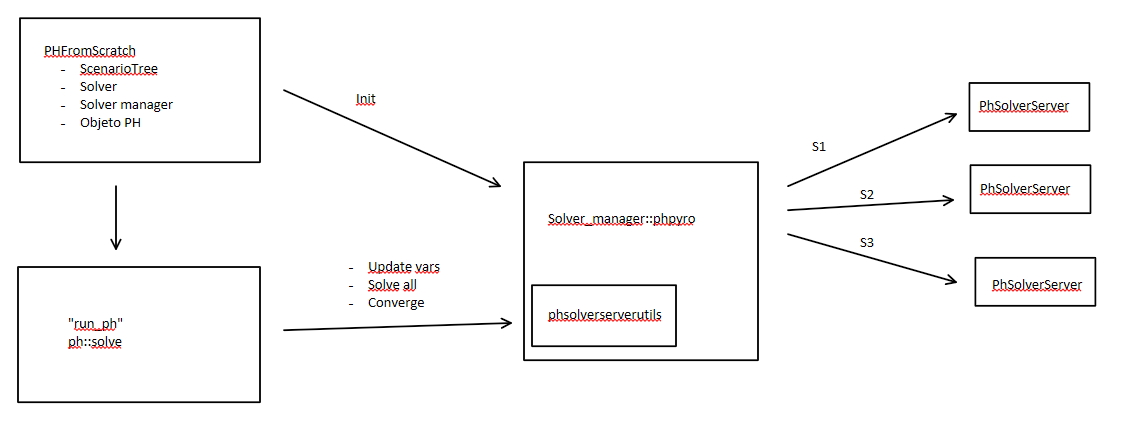
\includegraphics[width=15cm]{figuras/ph-diagram.png}}
    \caption{Diseño de runph}
    \label{fig:ph-diagram}
\end{figure}

Si tomamos el solver manager como el punto central, la parte de la derecha se ejecuta en paralelo, es decir, debemos implementarla en Spark; y la parte izquierda es la que genera los trabajos.\\

Teniendo en cuenta esta arquitectura y el tiempo disponible se propone una solución cuyo objetivo es aprovechar al máximo el código ya implementado en Pyomo y que facilite al máximo la integración de la nueva implementación. La solución propuesta es la creación de un nuevo solver manager que gestione los objetos \textit{PHSolverServer} como RDDs, donde se distribuyen los subproblemas. Con esto mantenemos el mismo sistema de ejecución mediante cola de tareas y sólo modificamos el gestor que las distribuye. 

% TODO: Intentar ampliar esto.
\cleardoublepage
\chapter{Implementación}
\label{ch:implementacion}

\section{Prototipo inicial}

% Este prototipo se utiliza para concretar el uso de Spark. Especificar las similitudes entre el prototipo implementado y la solución diseñada.

El objetivo de este primer prototipo es familiarizarse con el uso de Spark desde Python así como el manejo de una lista de objetos mediante un RDD.\\

Para que el prototipo sea de utilidad, sigue una arquitectura similar al diseño planteado para Pyomo. En este caso contamos con dos archivos distintos:

\begin{itemize}
    \item \textbf{main.py: } Representa las funciones del nuevo solver manager, gestionando la interacción con Spark y el envio de tareas a los workers.
    \item \textbf{worker.py: } Implementa el objeto que realizará el procesamiento de los datos. Representa a los objetos PHSolverServer.
\end{itemize}

En la \autoref{fig:prototipo} se muestra el código de \texttt{main.py}. En este prototipo vemos cómo conectarnos a una instancia de Spark utilizando el objeto \texttt{SparkConf}. A continuación creamos un RDD a partir de una lista de objetos utilizando el método \texttt{parallelize}.
La ejecución de cada iteración se hace iterando sobre los elementos del RDD, es decir, la lista de workers, mediante la función \texttt{map} e indicando una función como parámetro de la expresión lambda. Esto ejecuta una transformación sobre el RDD, ejecutando la función definida en cada elemento. 
Para que que esta transformación se llegue a ejecutar, es necesario utilizar una acción de Spark. En este prototipo, la acción realizada es \texttt{collect}, que nos devuelve una lista con los contenidos del RDD tras ejecutar las transformaciones anteriores.\\

\begin{figure}[]
    \centerline{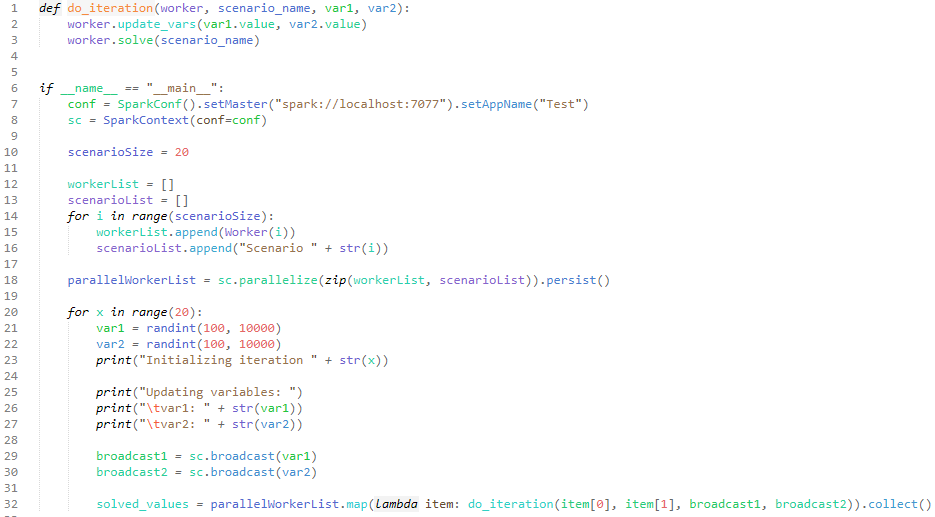
\includegraphics[width=15cm]{figuras/codigo/prototipo.png}}
    \caption{Prototipo inicial}
    \label{fig:prototipo}
\end{figure}

Los workers en este prototipo simplemente realizan un cierto número de operaciones aleatorias para simular un cierto tiempo de ejecución y comprobar si la ejecución de Spark se está realizando en paralelo y qué niveles de escalabilidad nos podemos esperar.

\section{Integración}

% Especificar cómo funciona la cola de tareas, su solicitud por parte del gestor y cómo se utiliza el RDD en este contexto.

La siguiente fase del prototipado es comenzar la implementación sobre el proyecto final. Este prototipo tiene como objetivo probar la integración con el proyecto y verificar que el flujo de ejecución es correcto.\\

El primer paso es crear el nuevo solver manager que denominaremos \textit{PHSpark}. Se crea una nueva clase en la ruta \textit{``/pyomo/pyomo/solvers/plugins/smanager''} y comenzamos copiando el código de phpyro. De esta forma nos aseguramos de mantener una interfaz común y sólo tendremos que cambiar la implementación de los métodos. 
Si queremos que la integración sea correcta, este solver manager debe poder seleccionarse como una opción de \texttt{runph} desde la línea de comandos. Para conseguir que funcione la opción \texttt{--solver-manager=phspark} debemos especificar ``phspark'' como nombre del plugin que será el nuevo solver manager. Esto se consigue usando el método \texttt{pyomo.util.plugin.alias(``phspark'')} en la definición de nuestro solver manager. También es necesario importarlo como parte del paquete de smanagers en el archivo \texttt{/plugins/smanager/\_\_init\_\_.py}.\\

La primera tarea que realizan los workers es la inicialización por lo que se establece como criterio de aceptación de este prototipo la ejecución correcta de esta tarea por parte de los workers (funcionando en Spark) y la devolución correcta de los resultados.\\

El primer paso es la creación del RDD. Esto se realiza mediante la función \texttt{acquire\_servers}. Como podemos ver en la \autoref{fig:code-acquire-servers-prototipo}, es una implementación muy similar al prototipo anterior. En este punto destaca la necesidad de cargar el archivo donde se encuentra la implementación de los solvers (\textit{phsolverserver.py}) en Spark. Si no cargamos este archivo manualmente se producirá un error porque el worker desde la instancia de Spark no puede resolver la dependencia. Este tipo de problemas serán comunes a lo largo de todo este proyecto. También cabe destacar la sustitución del serializador por defecto de pyspark. En este método estamos inicializando \texttt{CloudPickleSerializer} pues es necesario para serializar las funciones lambda que se pasarán como argumento al método \texttt{map} del RDD.\\

\begin{figure}[]
    \centerline{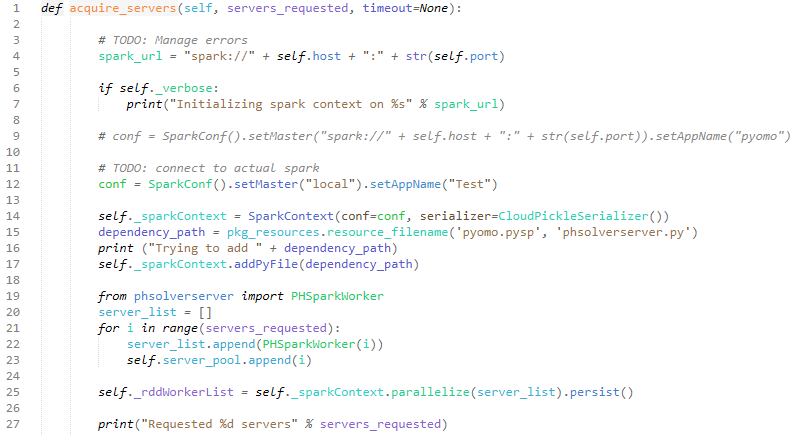
\includegraphics[width=15cm]{figuras/codigo/acquire-servers-prototipo.png}}
    \caption{Método acquire\_servers del prototipo de integración.}
    \label{fig:code-acquire-servers-prototipo}
\end{figure}

Una vez tenemos el RDD creado, el solver manager queda a la espera de que el hilo principal le ponga tareas en cola. Estas tareas son aceptadas en el método \texttt{\_perform\_queue}. Podemos ver la implementación inicial en la \autoref{fig:code-perform-queue-prototipo}. De nuevo, es muy similar al prototipo anterior. Se genera una tarea de Pyro y se envía a cada worker. La variable \texttt{queue\_name} indica a qué worker concreto está destinada la tarea y la usaremos para filtrar la ejecución. \\

\begin{figure}[]
    \centerline{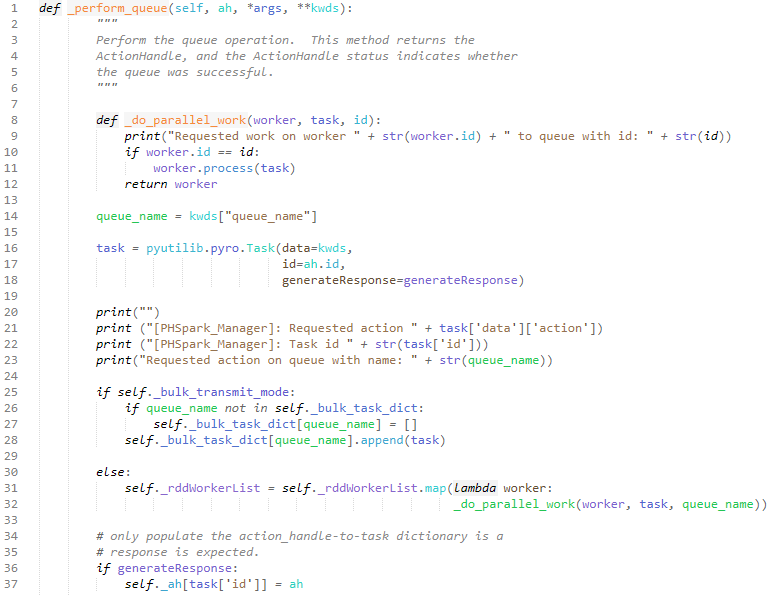
\includegraphics[width=15cm]{figuras/codigo/perform-queue-prototipo.png}}
    \caption{Método \_peform\_queue del prototipo de integración.}
    \label{fig:code-perform-queue-prototipo}
\end{figure}

Gracias a la evaluación perezosa de Spark, como en este método sólo realizamos una transformación sobre el RDD, podemos encadenar varias tareas y se ejecutarán cuando se solicite un resultado por parte del hilo principal.\\

En la implementación del worker, generamos un wrapper (\texttt{PHSparkWorker}) que encapsula el objeto \texttt{PHSolverServer} ya implementado. Este objeto pasará las tareas al objeto que encapsula y guarda los resultados en una lista privada. Cuando se solicite un resultado desde el hilo principal, se devolverán los resultados acumulados en esta lista hasta el momento. La implementación de este objeto se puede ver en la \autoref{fig:code-phsparkworker-prototipo}.\\

\begin{figure}[]
    \centerline{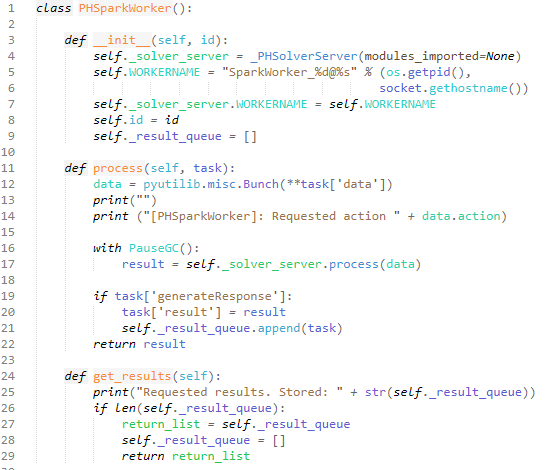
\includegraphics[width=15cm]{figuras/codigo/phsparkworker-prototipo.png}}
    \caption{Objeto PHSparkWorker del prototipo de integración.}
    \label{fig:code-phsparkworker-prototipo}
\end{figure}

Tras la inicialización del worker, debemos eliminar el parámetro \textit{scenario\_tree\_factory}, pues no es serializable e impide que se devuelvan los datos al hilo principal.

Con esta implementación conseguimos generar el RDD y ejecutar la tarea de inicialización satisfactoriamente. Aunque las siguientes iteraciones producen errores, el objetivo de este prototipo está cumplido con éxito y pasamos a la siguiente fase.

\section{Prototipo funcional}

% Utilización del map e ir explicando los problemas encontrados (serializador no compatible con lambdas, tener que devolver el propio worker junto al resultado, problemas de dependencias por rutas en los workers y el problema gordo). TODO: buscar en los informes de progreso información más concreta.

El esqueleto del nuevo solver manager ya está implementada y en esta fase nos centraremos en implementar lo necesario para que el algoritme finalice correctamente. En lugar de estar centrado en generar nuevo código, será una etapa donde se irán analizando los errores que aparezcan y solucionándolos. \\

Tras la finalización del anterior prototipo, observamos un error en las siguientes iteraciones del algoritmo. Este primer error sólo se trata de un problema de dependencias en el entorno de ejecución de Spark y se puede solucionar simplemente retrasando la importación del módulo \texttt{pyomo.environ} dentro del worker.\\

Esta primera versión llega a ejecutar las 100 iteraciones que tiene el algoritmo como máximo por defecto, pero acaba con un error. Si observamos el historial de convergencia que se imprime al final, los valores del algoritmo no avanzan. Sabemos que el algoritmo es diferente para la iteración 0 que para el resto y estamos observando que sólo la primera iteracion funciona correctamente. Encontramo que en los workers hay una variable que regula el comportamiento del \texttt{solve}, indicando si se encuentra en la primera iteración. Si seguimos su valor en las múltiples iteraciones, siempre estará como \texttt{True}, a pesar de que se le asigne expresamente el valor \texttt{False}. 
Una primera conclusión es la existencia de errores en la fase de serialización del RDD que, por alguna razón, impidan que este dato se guarde actualizado. Como no se encuentra el problema raiz, se fuerza el envío del número de iteración desde el hilo principal para poder avanzar. Con esto conseguimo que el algoritmo avance, pero converge en 33 iteraciones cuando debería llegar a la 100. El error en esta variable puede indicar que haya errores en otros datos que no persistan y esto supuso el primer retraso importante en el proyecto.\\

Este programa es bastante resistente frente a errores lo que implica que, aunque suceda un error, el programa puede continuar funcionando. Sin embargo, el resto de la ejecución, aunque no se pare, puede devolver resultados erróneos. Esto hace que encontrar errores sea bastante complicado.\\

Un problema recurrente en este proyecto son las dependencias. Al ser un proyecto con múltiples paquetes dependientes unos de otros, se hace complicado llevar uno de estos objetos a Spark. Cuando ejecutamos el objeto PHSolverServer dentro del entorno de Spark, aunque teóricamente se serializan sus dependencias, no accede correctamente a todos los archivos a los que tendría acceso en local.
En primer lugar, debemos hacer que el solver esté disponible para los workers. Como estamos usando el solver \textit{minos} que consta de un solo archivo ejecutable, es sencillo añadir este archivo únicamente como dependencia dentro de Spark mediante el método \texttt{addFile}. Para que los workers puedan utilizarlo deben conocer la ruta que tendrá este archivo en los nodos que se ejecuten. Para conseguir esta nueva ruta podemos utilizar la función de Spark \texttt{SparkFiles.get}. Por último debemos añadir el archivo que define el problema a solucionar, normalmente con el nombre de \textit{ReferenceModel.py}, pues se intenta añadir el archivo como un módulo y esto lo guarda con una ruta de acceso al archivo.\\

Otro caso de dependencias que debemos solucionar es el uso del patrón \textit{factory} desde dentro de Spark. Estas clases deben tener acceso a una lista de clases que pueden instanciar y esto puede no estar disponible desde un worker. La solución temporal a este problema es instanciar las clases necesarias para la ejecución fuera del RDD y luego pasar las instancias a los workers. Esto en principio limita las opciones que soporta nuestra nueva implementación, pues sólo tenemos acceso a un objeto para escribir archivos ``nl'', sólo podemos transformar modelos con ``mpec.nl'' y sólo podemos abrir soluciones en formato ``sol''. \\

Por último, observamos un problema en la creación del archivo necesario para la resolución del subproblema. Para generar este archivo se utiliza un objeto del tipo \texttt{ComponentMap} que contiene información sobre las variables del problema. Sin embargo, después de la primera iteración del solve, este objeto no tiene los datos correctos. Haciendo un seguimiento de sus contenidos, observamos que en el momento previo a la serialización, los contenidos son correctos, pero justo tras deserializar y comenzar la siguiente iteración, el objeto no se genera correctamente porque falta un atributo. Este atributo que falta es el \texttt{\_ampl\_repn} y, buscando en el código, se encontró lo siguiente en la función de serialización de uno de los objetos:

\begin{figure}[H]
    \centerline{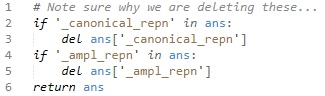
\includegraphics[width=10cm]{figuras/codigo/borrado-ampl.png}}
    \caption{Borrado del parámetro \_ampl\_repn.}
    \label{fig:ampl-repn-deletion}
\end{figure}

Una vez comentadas las líneas del segundo \textit{if}, podemos ejecutar el ejemplo ``Farmer'' y obtenemos el resultado correcto. En este punto consideramos el proyecto como funcionalmente correcto y damos esta fase como concluida.\\

En la \autoref{fig:code-acquire-servers-final} podemos ver cómo se inicializan los workers. Si lo comparamos con el anterior prototipo podemos ver una gestión de errores más completa y la instanciación de los workers se hace dentro de Spark (en lugar de paralelizar los objetos instanciados).\\

\begin{figure}[H]
    \centerline{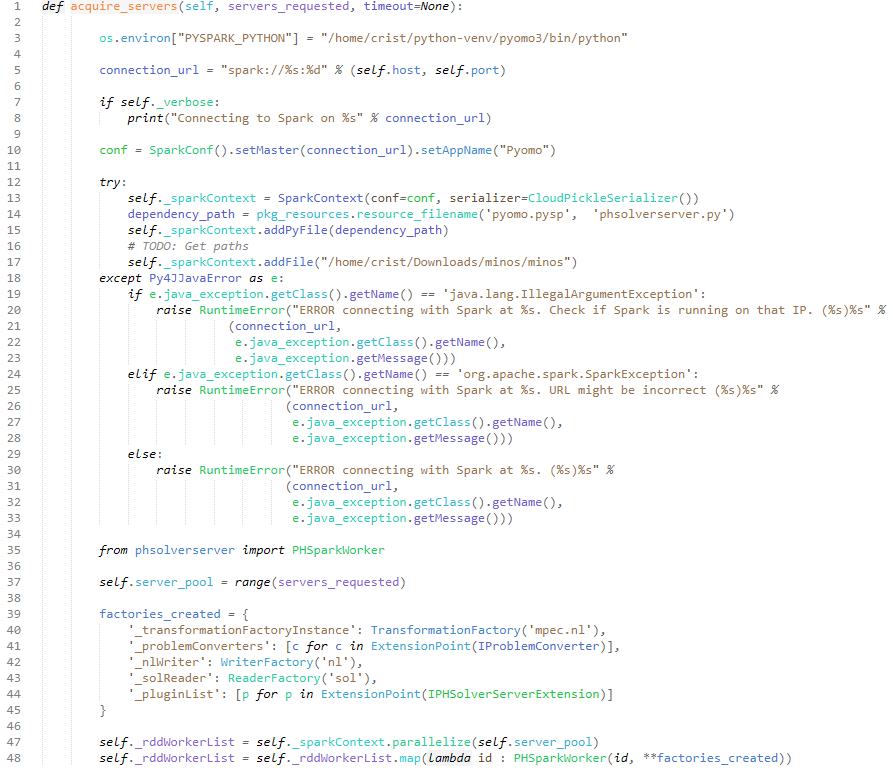
\includegraphics[width=15cm]{figuras/codigo/acquire-servers-final.png}}
    \caption{Método acquire\_servers del prototipo funcional.}
    \label{fig:code-acquire-servers-final}
\end{figure}

En el método de asignación de tareas (\autoref{fig:code-perform-queue-final}) no hay demasiadas diferencias con el anterior. La principal adición está en la ruta relativa del ejecutable del solver dentro de Spark, que se pasa como un keyword de la tarea ``initialize''.\\

\begin{figure}[H]
    \centerline{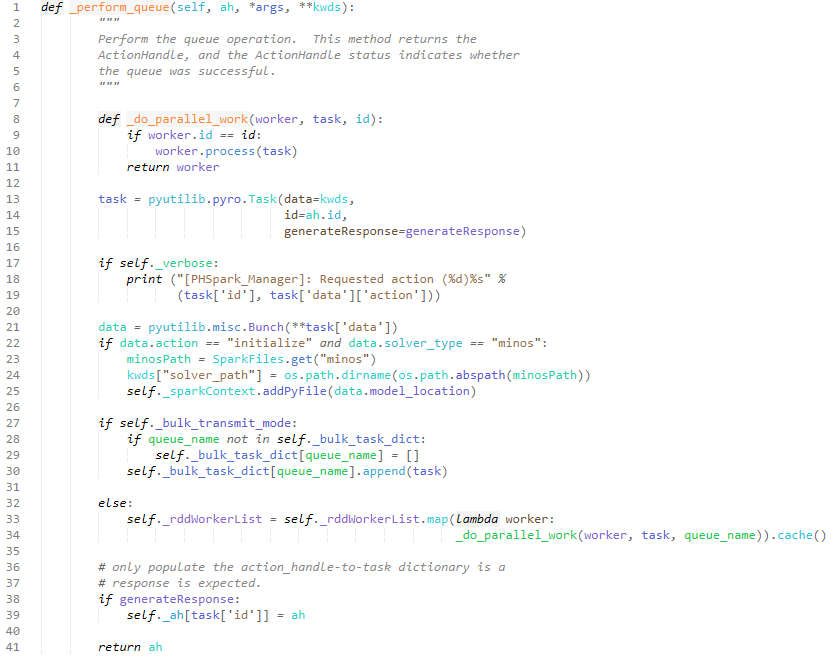
\includegraphics[width=15cm]{figuras/codigo/perform-queue-final.png}}
    \caption{Método \_peform\_queue del prototipo funcional.}
    \label{fig:code-perform-queue-final}
\end{figure}

El último método que merece explicación adicional es el encargado de la recolección de resultados desde Spark (\autoref{fig:code-wait-final}). Como estamos trabajando con un algoritmo iterativo, siempre que se realice una transformación sobre el RDD debemos mantener las instancias de \texttt{PHSparkWorker} actualizadas. En este caso, cuando realicemos la transformación en el RDD, queremos devolver la lista de resultados pendientes, pero también es necesario devolver el worker actualizado. Para conseguirlo, transformamos el RDD en un RDD formado por tuplas con el worker actualizado y sus resultados pendientes. Ahora filtramos esta tupla dos veces: primero cogemos sólo los resultados pendientes y los devolvemos al manager y luego cogemos sólo los workers actualizados para tener el RDD correcto en la siguiente iteración.

\begin{figure}[H]
    \centerline{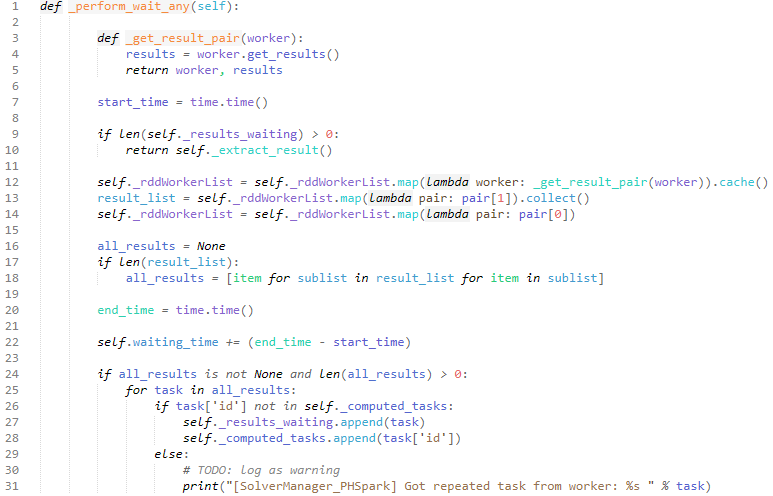
\includegraphics[width=15cm]{figuras/codigo/wait-final.png}}
    \caption{Método \_peform\_wait\_any del prototipo funcional.}
    \label{fig:code-wait-final}
\end{figure}
\cleardoublepage
\chapter{Plan de pruebas}
\label{sec:pruebas}

\section{Pruebas funcionales}

\subsection{Introducción}

El actual plan de pruebas tiene como objetivo asegurar que los requisitos especificados son cumplidos satisfactoriamente por el módulo de código implementado. Adicionalmente se buscará que el código implementado funcione correctamente cuando dispone de entradas incorrecta.

Este plan de pruebas está basado en el estándar IEEE 829 \cite{IEEE829}.

\subsection{Restricciones}

La principal restricción de este plan de pruebas es el tiempo. Sólo se dispone de 1 día para la creación del plan y otro día para su ejecución y la recolección de resultados.\\

La complejidad de las entradas que recibe el módulo limita el alcance de las pruebas de caja negra que podremos diseñar en el tiempo disponible.

\subsection{Objeto de pruebas}

El código a probar será la implementación del gestor de Spark, concretamente la clase {\it SolverManager\_PHSpark}. Su ejecución se realiza mediante el comando {\it runph} con la opción {\it -\-solver-manager=phspark}.\\

Se realizarán pruebas de caja negra sobre las diferentes opciones de configuración del solver manager. Adicionalmente se ejecutarán los ejemplos existentes en el proyecto y se comparará la solución generada mediante spark y mediante el algoritmo secuencial.

\subsection{Características a probar y exclusiones}

Se probarán las diferentes opciones de configuración que modifican la ejecución de phspark. Con esto verificamos el requisito RF-01 y RF-02.\\

Adicionalmente se ejecutan los ejemplos existentes para PySP mediante phspark y la implementación secuencial, comparando los resultados. De esta forma se verifica un funcionamiento correcto en distintos escenarios así como el requisito RF-03.\\

Queda excluído de este plan de pruebas la generación de pruebas mediante estrategias de caja blanca. No podremos asegurar una cobertura óptima de código pero no es posible realizarlas en el tiempo disponible dada la complejidad de las entradas.

\subsection{Estrategia}

Se utilizará el módulo ``unittest'' de Python para generar una clase que ejecute los casos de prueba diseñados.\\

Será necesario generar un archivo de salida correcto para usar como punto de comparación con las ejecuciones de pruebas. Será necesario filtrar las diferencais en la salida que causa la ejecución con Spark o, alternativamente, comprobar manualmente el resultado de cada pareja de archivos.

\subsection{Criterios de aceptación}

Se considerará que una prueba ha sido pasada correctamente si, tras introducir los datos de entrada escogidos, la aplicación devuelve una salida que concuerda exactamente con la que se estableció como esperada.\\

Será posible concluir que la aplicación aprobada pasó las pruebas si el 100\% de los casos válidos pasaron los criterios de aceptación. En caso contrario será necesaria la corrección de la implementación.

\subsection{Diseño de pruebas}

\TestItem[
    id={P-01},
    name={Conexión a Spark},
    requirements={RF-01, RF-02},
    objective={
        Valida la creación de una conexión a Spark.
    },
    techniques={
        \begin{itemize}
            \item \textbf{Por caja negra: }
            \begin{itemize}
                \item host
                \begin{itemize}
                    \item 1. Clase válida: Cadena que represente una IP correcta y disponible.
                    \item 2. Clase válida: Null.
                    \item 3. Clase no válida: Cadena que represente una IP errónea.
                    \item 4. Clase no válida: Cadena que represente una IP correcta pero no disponible.
                \end{itemize}
                \item port 
                \begin{itemize}
                    \item 5. Clase válida: Entero que represente un puerto correcto y disponible.
                    \item 6. Clase válida: Null.
                    \item 7. Clase no válida: Entero que represente un puerto erróneo.
                    \item 8. Clase no válida: Entero que represente un puerto correcto pero ocupado.
                \end{itemize}
            \end{itemize}
        \end{itemize}
    },
    testCases={CP-01, CP-02, CP-03, CP-04, CP-05, CP-06},
    expected={Conexión correcta y ejecución que genere la salida esperada en el caso de las pruebas para clases válidas. Para las pruebas con entradas no válidas se debe mostrar un error especificando el problema.}
]

\TestItem[
    id={P-02},
    name={Ejecución correcta de ejemplos},
    requirements={RF-01, RF-02, RF-03},
    objective={
        Valida que los resultados devueltos son correctos.
    },
    techniques={
        Se ejecutarán todos los ejemplos disponibles en \textit{``/pyomo/examples/pysp''} usando la versión secuencial para generar el resultado esperado y la versión Spark para verificar su funcionamiento.
    },
    testCases={CP-01, CP-02, CP-03},
    expected={Los resultados de todos los ejemplos son iguales para la versión secuencial y paralela.}
]

\subsection{Casos de prueba}

\TestCase[
    id={CP-01},
    description={Prueba la entrada correcta},
    validates={P-01(1,5)},
    environment={
        Instancia de Spark funcionando en ``spark://localhost:7077''
    },
    input={
        \makecell{
            host = ``localhost''\\
            port = 7077
        }
    },
    output={
        Igual a la ejecución con -\-solver-manager=serial
    }
]

\TestCase[
    id={CP-02},
    description={Prueba la url por defecto},
    validates={P-01(2,6)},
    environment={
        Instancia de Spark funcionando en ``spark://localhost:7077''
    },
    input={
        \makecell{
            host = None\\
            port = None
        }
    },
    output={
        Igual a la ejecución con -\-solver-manager=serial
    }
]

\TestCase[
    id={CP-03},
    description={Prueba la gestión de error al intentar conectarse a una IP incorrecta},
    validates={P-01(3)},
    environment={
        N/A
    },
    input={
        \makecell{
            host = ``111.111''\\
            port = None
        }
    },
    output={
        Mensaje de error indicando que no se ha podido conectar a Spark en la URL especificada.
    }
]

\TestCase[
    id={CP-04},
    description={Prueba la gestión de error al intentar conectarse a una IP donde no se está ejecutando Spark},
    validates={P-01(4)},
    environment={
        La URL ``spark://localhost:7077'' no debe tener ningún servicio escuchando.
    },
    input={
        \makecell{
            host = ``localhost''\\
            port = 7077
        }
    },
    output={
        Mensaje de error indicando que no se ha podido conectar a Spark en la URL especificada.
    }
]

\TestCase[
    id={CP-05},
    description={Prueba la gestión de error al especificar un puerto inválido},
    validates={P-01(7)},
    environment={
        N/A
    },
    input={
        \makecell{
            host = None\\
            port = -1
        }
    },
    output={
        Mensaje de error indicando que no se ha podido conectar a Spark en la URL especificada.
    }
]

\TestCase[
    id={CP-06},
    description={Prueba la gestión de error al especificar un puerto donde no se está ejecutando Spark},
    validates={P-01(8)},
    environment={
        La URL ``spark://localhost:8080'' no debe ser una instancia de Spark
    },
    input={
        \makecell{
            host = ``localhost''\\
            port = 8080
        }
    },
    output={
        Mensaje de error indicando que no se ha podido conectar a Spark en la URL especificada.
    }
]

\subsection{Procedimiento de pruebas}

Los casos de prueba especificados son idempotentes y no es necesario especificar un orden concreto para su ejecución. Será necesario para cada uno establecer el entorno especificado en cada caso concreto. Adicionalmente, para verificar los resultados será necesario ejecutar la misma entrada de forma secuencial para comparar.\\

Para la prueba P-02 no se especifican casos de prueba concretos porque todos se ejecutan de la misma forma cambiando el directorio de entrada. Para esta prueba se ejecutarán todos los ejemplos disponibles para PySP de forma secuencial y, posteriormente, usando Spark. Si Spark devuelve siempre los mismos resultados (dentro de un margen de error) se considerará la prueba como superada.

\subsection{Ejecución de las pruebas}

Por limitaciones temporales, los tests unitarios no están totalmente automatizados. Actualmente, la arquitectura de tests necesita de la creación de archivos de referencia para contrastar con la salida de la ejecución de prueba. Adicionalmente, por las posibles diferencias entre ambos archivos no relevantes para el resultado (como mensajes informativos), se debe programar un filtro concreto para las diferentes salidas.\\

Por las razones expuestas los tests se programarán para ejecutarse automáticamente, pero se debe comprobar manualmente si la salida es la esperada. Para realizar esta comprobación se ejecutará el mismo comando que ejecuta cada test, pero utilizando {\it --solver-manager=serial}.\\

La solución de cada ejecución se guarda en un archivo \textit{ph\_solution.json}. Se guarda la solución de la ejecución secuencial y posteriormente es posible ejecutar \textit{diff} con la solución devuelta por el test, siempre que se espere una salida correcta. En caso contrario se comprobará manualmente que la salida es la esperada.\\

\begin{tabularx}{\linewidth}{|c|X|c|}
    \hline
    \textbf{ID} & \centering \textbf{Salida} & \textbf{Superada} \tabularnewline
    \hline
    CP-01 & TestPHFarmerSpark.test1.ph\_solution.json.out & Si \tabularnewline
    \hline
    CP-02 & TestPHFarmerSpark.test2.ph\_solution.json.out & Si \tabularnewline
    \hline
    CP-03 & RuntimeError: ERROR connecting with Spark at spark://111.111:7077. URL might be incorrect (org.apache.spark.SparkException)Invalid master URL: spark://111.111:7077 & Si \tabularnewline
    \hline
    CP-04 & RuntimeError: ERROR connecting with Spark at spark://192.10.10.10:7077. Check if Spark is running on that IP. (java.lang.IllegalArgumentException)requirement failed: Can only call getServletHandlers on a running MetricsSystem & Si \tabularnewline
    \hline
    CP-05 & RuntimeError: ERROR connecting with Spark at spark://localhost:-1. URL might be incorrect (org.apache.spark.SparkException)Invalid master URL: spark://localhost:-1 & Si \tabularnewline
    \hline
    CP-06 & RuntimeError: ERROR connecting with Spark at spark://localhost:8080. Check if Spark is running on that IP. (java.lang.IllegalArgumentException)requirement failed: Can only call getServletHandlers on a running MetricsSystem & Si \tabularnewline
    \hline
\end{tabularx}

A continuación se probará la ejecución de los ejemplos disponibles en el proyecto. Para ello se utilizará un script en bash que se mueva entre los directorios y ejecute la versión secuencial y paralela para cada ejemplo, imprimiendo los resultados de ejecutar el comando \textit{diff}. Aunque con este script se busca automatizar al máximo la ejecución de pruebas, no se consigue totalmente. La naturaleza del algoritmo hace que existan ligeras diferencias en los valores generados. Esto causará que las salidas sean diferentes, pero no implica que los resultados sean incorrectos. 
Para facilitar la comprobación de esta situación, se utiliza la herramienta \textit{colordiff} que resaltará las diferencias entre ambas soluciones.\\

A continuación se muestra el primer test del script donde se ejecuta el ejemplo ``Farmer''. La ejecución de los ejemplos restantes es equivalente, modificando únicamente las rutas de los archivos.\\

\begin{figure}[H]
    \centerline{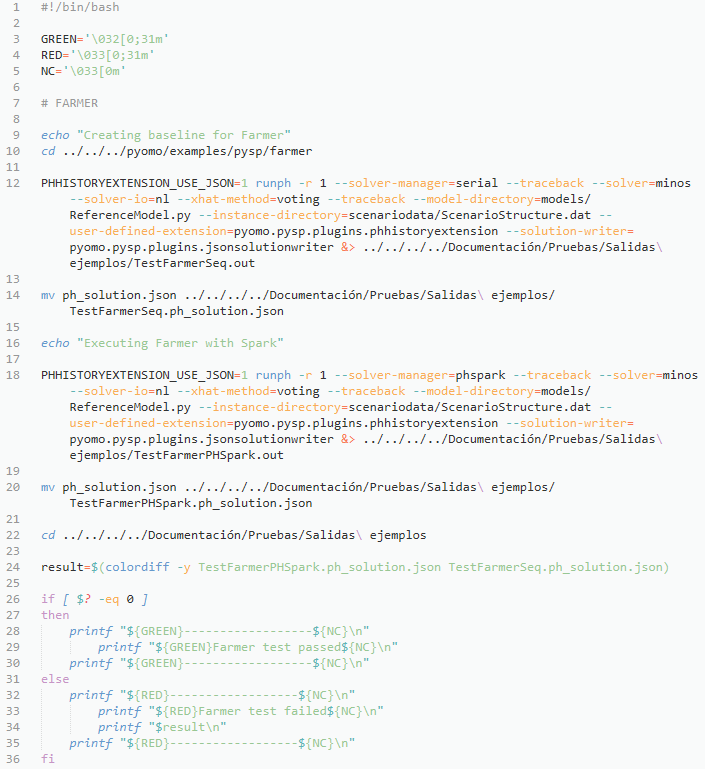
\includegraphics[width=15cm]{figuras/codigo/script-pruebas.png}}
    \caption{Script de pruebas}
\end{figure}

El resultado de ejecutar este script completo se muestra en la tabla a continuación: \\

\begin{tabularx}{\linewidth}{|X|c|}
    \hline
    Farmer & passed \tabularnewline
    \hline
    Baa99 & failed (stackoverflow) \tabularnewline
    \hline
    Farmer\_generated & failed (stackoverflow) \tabularnewline
    \hline
    FarmerWIntegers & passed \tabularnewline
    \hline
    FarmerWPieceWise & passed \tabularnewline
    \hline
    FarmerWrent & passed \tabularnewline
    \hline
    Finance & failed (stackoverflow) \tabularnewline
    \hline
    Hydro & passed \tabularnewline
    \hline
\end{tabularx}
\\ \newline
Podemos observar que algunos tests aparecen como fallidos con un error \textit{stackoverflow}. Esto no significa necesariamente que el programa no funcione como se espera, lo más probable es que se deba a limitaciones de la máquina en la que se han realizado las pruebas.\\

Queda como tarea en un futuro optimizar la gestión de la memoria y el uso de Spark para que ejecutar problemas como este sea posible en máquinas con menos recursos. 

\section{Pruebas de rendimiento}

\subsection{Introducción}

\subsection{Restricciones}

\subsection{Objeto de pruebas}

\subsection{Características a probar y exclusiones}

\subsection{Estrategia}

\subsection{Criterios de aceptación}

\subsection{Diseño de pruebas}

\subsection{Casos de prueba}

\subsection{Procedimiento de pruebas}

\subsection{Ejecución de las pruebas}
\cleardoublepage
\chapter{Conclusiones}
\label{ch:conclusiones}

\section{Lecciones aprendidas}

\section{Trabajo futuro}

% Aquí empezan os apéndices
\appendix
\cleardoublepage
\chapter{Manual de despliegue}

En esta sección se explicará como instalar Spark y ejecutar los ejemplos incluidos en Pyomo con el nuevo módulo \texttt{phspark}.

El primer paso será descargar la distribución de Spark para nuestro sistemas operativo desde la página oficial (\url{http://spark.apache.org/downloads.html}). En el momento de realización de este documento, la última versión es la 2.3.1. Una vez descargado, podemos iniciarlo con la configuración por defecto ejecutando el script \texttt{/sbin/start-all.sh}.

Podemos comprobar que Spark se ha iniciado correctamente accediendo a la interfaz web en \texttt{localhost:8080}, como se ve en la \autoref{fig:manual-spark-web}. En este caso, para acceder al clúster, usaremos la url \texttt{localhost:7077} y esa será la dirección que le indicaremos a Pyomo.\\

\begin{figure}[H]
    \centerline{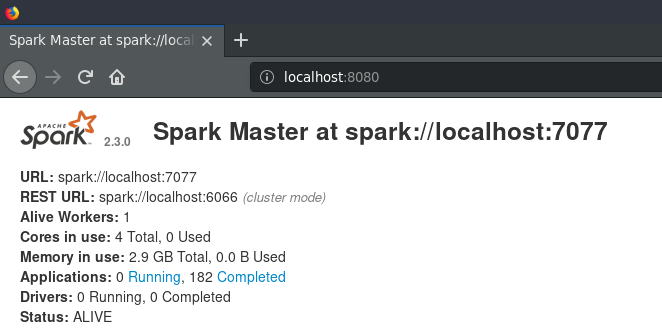
\includegraphics[width=15cm]{figuras/manual/spark-web-interface.png}}
    \caption{Interfaz web de Spark}
    \label{fig:manual-spark-web}
\end{figure}

Teniendo Python 3.6 instalado, vamos a la carpeta raíz del proyecto Pyomo. En esta carpeta hay un archivo \texttt{setup.py}. Para instalar este repositorio de Pyomo como librería en nuestro Python actual, ejecutamos: \\

\texttt{python setup.py develop}. \\

En caso de necesitar librerías adicionales se instalarán usando \texttt{pip}. Algunos requisitos probables son \textit{Pyro} y \textit{Pyutillib}.\\

Con este entorno instalado ya podemos ejecutar los ejemplos de Pyomo utilizando \texttt{phspark}. Para ello, nos movemos a la carpeta \texttt{/pyomo/examples/pysp/farmer} y ejecutamos el siguiente comando:\\

\begin{verbatim}
    runph -r 1 --solver-manager=phspark --traceback --solver=minos
     --solver-io=nl --xhat-method=voting --verbose 
     --model-directory=models/ReferenceModel.py 
     --instance-directory=scenariodata/ScenarioStructure.dat  
     --spark-host=localhost --spark-port=7077
\end{verbatim}

Esto nos mostrará la traza de ejecución y los resultados del problema al final.

\cleardoublepage
\chapter{Licenza}
Se se quere pór unha licenza (GNU GPL, Creative Commons, etc), o texto da licenza vai aquí.


\cleardoublepage
\markboth{BIBLIOGRAFÍA}{BIBLIOGRAFÍA}
\addcontentsline{toc}{chapter}{Bibliografía}


\begin{thebibliography}{99}
% % EXEMPLO DE DOCUMENTO DESCARGADO DA WEB
% \bibitem{cuda} Nvidia CUDA programming guide. Versión 2.0, 2010. Dispoñible en % {\it http://www.nvidia.com}.
% 
% % EXEMPLO DE PÁXINA DA WIKIPEDIA
% \bibitem{cdma} Acceso múltiple por división de código. Artigo da wikipedia (% {\it http://es.wikipedia.org}). Consultado o 2 de xaneiro do 2010.
% 
% % EXEMEPLO DE LIBRO
% \bibitem{gonzalez} R.C. Gonzalez e R.E. Woods, {\it Digital image processing}, % 3ª edición, Prentice Hall, New York, 2007.
% 
% % EXEMPLO DE ARTIGO DE REVISTA
% \bibitem{patricia} P. González, J.C. Cartex e T.F. Pelas, ``Parallel % computation of wavelet transforms using the lifting scheme'', {\it Journal of % Supercomputing}, vol. 18, no. 4, pp. 141-152, junio 2001.

\bibitem{learningSpark} Matei Zaharia, Patrick Wendell, Andy Konwinski, Holden Karau, {\it Learning Spark: Lightning-Fast Big Data Analysis}, 1ª edición, O'Reilly Media, 2015.

\bibitem{stochasticProgramming} John R. Birge, François Louveaux, {\it Introduction to Stochastic Programming}, 2ª Edición, Springer, 2011.

\bibitem{IEEE829} IEEE Std 829-2008, IEEE Standard for Software and System Test Documentation

% Files local to the project

\bibitem{local_funcionamientoPH} PONER AQUÍ LA RUTA
\bibitem{local_distributedTestApp} Proyecto de pruebas en: ``/DistributedTest''

\end{thebibliography}



\end{document}
